%%%%%%%%%%%%%%%%%%%%%%%%%%%%%%%%%%%%%%%%%%%%%%%%%%%%%%%%%%%%%%%%%%%%%%%%%%%%%%%%
%%%%%%%%%%%%%%%%%%   Vorlage für eine Abschlussarbeit   %%%%%%%%%%%%%%%%%%%%%%%%
%%%%%%%%%%%%%%%%%%%%%%%%%%%%%%%%%%%%%%%%%%%%%%%%%%%%%%%%%%%%%%%%%%%%%%%%%%%%%%%%

% Erstellt von Maximilian Nöthe, <maximilian.noethe@tu-dortmund.de>
% ausgelegt für lualatex und Biblatex mit biber

% Kompilieren mit
% latexmk --lualatex --output-directory=build thesis.tex
% oder einfach mit:
% make
 
\documentclass[
  tucolor,       % remove for less green,
  BCOR=12mm,     % 12mm binding corrections, adjust to fit your binding
  parskip=half,  % new paragraphs start with half line vertical space
  open=any,      % chapters start on both odd and even pages
  cleardoublepage=plain,  % no header/footer on blank pages
]{tudothesis}

% Warning, if another latex run is needed
\usepackage[aux]{rerunfilecheck}

% just list chapters and sections in the toc, not subsections or smaller
\setcounter{tocdepth}{1}

%------------------------------------------------------------------------------
%------------------------------ Fonts, Unicode, Language ----------------------
%------------------------------------------------------------------------------
\usepackage{fontspec}
\defaultfontfeatures{Ligatures=TeX}  % -- becomes en-dash etc.

% load english (for abstract) and ngerman language
% the main language has to come last
\usepackage[american, ngerman]{babel}

% intelligent quotation marks, language and nesting sensitive
\usepackage[autostyle]{csquotes}

% microtypographical features, makes the text look nicer on the small scale
\usepackage{microtype}

%------------------------------------------------------------------------------
%------------------------ Math Packages and settings --------------------------
%------------------------------------------------------------------------------

\usepackage{amsmath}
\usepackage{amssymb}
\usepackage{mathtools}

% Enable Unicode-Math and follow the ISO-Standards for typesetting math
\usepackage[
  math-style=ISO,
  bold-style=ISO,
  sans-style=italic,
  nabla=upright,
  partial=upright,
]{unicode-math}
\setmathfont{Latin Modern Math}

% nice, small fracs for the text with \sfrac{}{}
\usepackage{xfrac}


%------------------------------------------------------------------------------
%---------------------------- Numbers and Units -------------------------------
%------------------------------------------------------------------------------

\usepackage[
  locale=DE,
  separate-uncertainty=true,
  per-mode=symbol-or-fraction,
]{siunitx}
% \sisetup{math-micro=\text{µ},text-micro=µ} % has been removed

%------------------------------------------------------------------------------
%-------------------------------- tables  -------------------------------------
%------------------------------------------------------------------------------

\usepackage{booktabs}       % \toprule, \midrule, \bottomrule, etc

%------------------------------------------------------------------------------
%-------------------------------- graphics -------------------------------------
%------------------------------------------------------------------------------

\usepackage{graphicx}
\graphicspath{ {./plots/}{./graphics/} }
% currently broken
% \usepackage{grffile}

% allow figures to be placed in the running text by default:
\usepackage{scrhack}
\usepackage{float}
\floatplacement{figure}{htbp}
\floatplacement{table}{htbp}

% keep figures and tables in the section
\usepackage[section, below]{placeins}


%------------------------------------------------------------------------------
%---------------------- customize list environments ---------------------------
%------------------------------------------------------------------------------

\usepackage{enumitem}

%------------------------------------------------------------------------------
%------------------------------ Bibliographie ---------------------------------
%------------------------------------------------------------------------------

\usepackage[
  backend=biber,   % use modern biber backend
  autolang=hyphen, % load hyphenation rules for if language of bibentry is not
                   % german, has to be loaded with \setotherlanguages
                   % in the references.bib use langid={en} for english sources
]{biblatex}
\addbibresource{references.bib}  % the bib file to use
\DefineBibliographyStrings{german}{andothers = {{et\,al\adddot}}}  % replace u.a. with et al.


% Last packages, do not change order or insert new packages after these ones
\usepackage[pdfusetitle, unicode, linkbordercolor=tugreen, citebordercolor=tugreen]{hyperref}
\usepackage{bookmark}
\usepackage[shortcuts]{extdash}

%------------------------------------------------------------------------------
%------------------------------ own imports -----------------------------------
%------------------------------------------------------------------------------

% \usepackage[smartEllipses]{markdown}
\usepackage{xcolor}
\newcommand\marktodo[1]{\textcolor{red}{#1}}
\usepackage{incgraph,tikz}
% \usepackage[hashEnumerators,smartEllipses]{markdown}
\usepackage{enumitem}


%------------------------------------------------------------------------------
%-------------------------    Angaben zur Arbeit   ----------------------------
%------------------------------------------------------------------------------

\author{Martin Schönfeld}
\title{PROPOSAL-Simulationsstudien zur Myographie in stillgelegten Bergbaustollen}
\date{2022}
\birthplace{Neustadt a.d.Aisch}
\chair{Lehrstuhl für Experimentelle Physik V}
\division{Fakultät Physik}
\thesisclass{Bachelor of Science}
\submissiondate{19. Mai 2022}
\firstcorrector{Prof.~Dr.~Dr.~Wolfgang Rhode}
\secondcorrector{Prof.~Dr.~Kevin Kröninger}

% tu logo on top of the titlepage
\titlehead{
\includegraphics[height=1.5cm]{logos/tu-logo.pdf}}

\begin{document}
\frontmatter
% \input{content/hints.tex}
\maketitle 
 
% Gutachterseite
\makecorrectorpage

% hier beginnt der Vorspann, nummeriert in römischen Zahlen
% \input{content/00_abstr.tex}
\tableofcontents

\mainmatter
% Hier beginnt der Inhalt mit Seite 1 in arabischen Ziffern

\chapter{Einleitung}
% \marktodo{Lieber Korrekturlesende! Zur Erklärung: Die roten Schriften sind Notizen an mich selbst von todos etc., nicht wundern.} 

% Hier folgt eine kurze Einleitung in die Thematik der Bachelorarbeit.
% Die Einleitung muss kurz sein, damit die vorgegebene Gesamtlänge der 
% Arbeit von 25 Seiten nicht überschritten wird. 
% Die Beschränkung der Seitenzahl sollte man ernst nehmen,
% da Überschreitung zu Abzügen in der Note führen kann. 
% Um der Längenbeschränkung zu genügen, darf auch nicht an der Schriftgröße,
% dem Zeilenabstand oder dem Satzspiegel (bedruckte Fläche der Seite) manipuliert werden.

Das Ruhrgebiet ist aus historischer Sicht für den Bergbau bekannt.
% Heutzutage gibt es im Ruhrgebiet keinen aktiven- oder Steinkohleabbau
% mehr\footnote{Das letzte Steinkohlebergwerk Prosper-Haniel Bottrop schloss am.
% 21. Dezember 2018.}.
Heutzutage gibt es im Ruhrgebiet allerdings keinen aktiven Braun- oder Steinkohleabbau
mehr\footnote{Das letzte Steinkohlebergwerk Prosper-Haniel Bottrop schloss am.
21. Dezember 2018.}.

Beim Bau und während der Benutzung musste rund um die Uhr mit Pumpen dafür gesorgt werden,
dass die Stollen nicht überfluten. Jene Bodenschichten besitzen von Natur aus ein 
gewisses Hohlraumvolumen, welches naturgemäß mit Wasser gefüllt ist.

Trotz sukzessiver Stilllegung der Bergwerke in den letzten Jahrzehnten
muss allerdings weiterhin der Wasserstand der Stollen mit Pumpen unter Kontrolle gehalten werden.
Dies geschieht aus zwei Gründen: \\
Zum einen ist durch den massiven Bergbau im Ruhrgebiet im Laufe des letzten Jahrhunderts 
das Ruhrgebiet allmählich abgesackt und unter den Grundwasserspiegel gesunken. 
Ein Vernachlässigen der Wasserstände hätte zur Konsequenz, dass ganze Städte überflutet würden 
(siehe Abb. \ref{fig:Ruhrgebiet_Seen}). Zum anderen sind Verschmutzungen des Grubenwassers
\footnote{Verschmutzungen Steinkohlenbergwerke z.B.: Nickelsulfat, Eisenoxide und Mangan.\cite{grubenwasser}}
\footnote{Verschmutzungen Braunkohlenbergwerke z.B.: Kalzium, Eisenmonoxid, Zink, Magnesium,
 Natrium, Ammonium und Mangan \cite{grubenwasser}}.
Es soll verhindert werden, dass das Grubenwasser unser Grundwasser
und somit teilweise auch das Trinkwasser verschmutzt.


Die Forschungsfrage dieser Arbeit ist es herauszufinden, inwiefern mithilfe der Myographie 
der Wasserstand in einem stillgelegten Bergbaustollen gemessen werden kann. 

Es wird die Zählrate eines Detektors am Boden einer Bohrung simuliert.
Aus den Informationen der Bohrung wird als Fundament für die Simulation 
ein Bodenmodell erstellt.
Es werden verschiedene Wasserhöhen aus den für den Bergbau drainierten Bodenschichten modelliert.
Es wird untersucht, wie sensitiv die Zählrate des Detektors auf veränderliche Wasserstände ist. 
\\
Der Myonenfluss wird mit EcoMug bestimmt und die Myonen mit PROPOSAL simuliert.

\begin{figure}[]
   \centering
   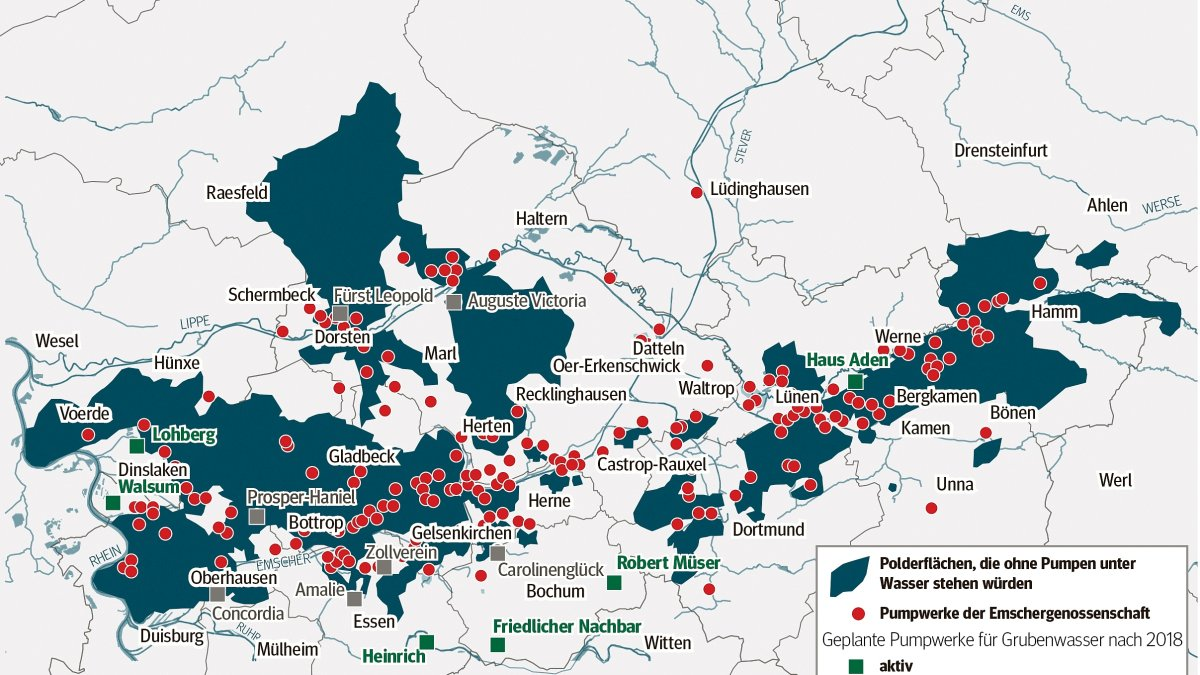
\includegraphics[width=\textwidth]{ruhrgebiet_unter_wasser.jpg}
   \caption{In Dunkelblau die Regionen im Ruhrgebiet, welche aufgrund der Absenkungen 
   unter Wasser stehen würden, wenn nicht ständig gepumpt werden würde. 
   2019 betrugen sich die Kosten für die Pumpwerke auf 220 Millionen Euro\cite{waz_seen}}
   \label{fig:Ruhrgebiet_Seen}
\end{figure}

% Zum Schluss wir die Simulation auf einen Detektor übertragen und 
% Messzeiten für eine Detektor ausgerechnet.

%  \marktodo{
%     - noch einen vergleich zu konventionellen methoden und was vorteile der myopgrahie sind???
%     }
\chapter{Theoretische Grundlage}
\label{sec:theorie}

% Dieser Abschnitt erklärt was Atmospärische Myonen sind
% und warum sie in der Myographie angewandt werden.
% Danach wird die Funktionsweise der Myographie erklärt,
% sowie deren Anwendungsbeispiele.

% solange nicht umstruturiert:
Dieser Abschnitt behandelt die theoretischen Grundlagen der Myographie.
Als Erstes werden atmosphärische Myonen vorgestellt, auf deren Absorption
die Myographie basiert. 

\section{Atmosphärische Myonen}

Myonen sind geladene Leptonen mit einer Ruhemasse von 
$m_{0} \approx \SI[]{106}[]{MeV}$ 
\cite{PDG2020}
und werden in der Atmosphäre aus der 
geladenen kosmischen Strahlung erzeugt (deshalb auch
kosmische Myonen genannt).
%  \marktodo{woraus besteht kosmische strahlung} 
Die kosmische Strahlung besteht im Allgemeinen aus hochenergetischen Teilchen,
welche von der Sonne, der Milchstraße oder fernen Galaxien kommt.
Die kosmische Strahlung ist beschreibbar über das Potenzgesetz   
\begin{equation*}
    \frac{\mathrm{d}N}{\mathrm{d}E}\thicksim E^{-\gamma}.
\end{equation*}
$N$ steht für die Anzahl an Teilchen und $E$ für die Energie.
$\gamma$ ist der sog. \textit{spektrale Index}. 
Für $E \leq 10^{15,5}\,\mathrm{eV}$ gilt $\gamma = \num{2,7}$ \cite{Gaisser16CR}. 

Die geladene kosmische Strahlung wechselwirkt mit den Stickstoff-, Sauerstoff- und 
Argonatomen in der Erdatmosphäre und erzeugt Luftschauer bestehend aus Hadronen, 
einem elektromagnetischen Teil, sowie Myonen.

Zur Produktion der Myonen wird zwischen den konventionellen 
und prompten Myonen unterschieden \cite{Gaisser16CR}.
Konventionelle Myonen entstehen aus Zerfällen von Pionen und Kaonen:
\begin{align*}
    \pi^{+} \to \mu^{+} + \nu_{\mu},\quad  & K^{+} \to \mu^{+} + \nu_{\mu}, \\
    \pi^{-} \to \mu^{-} + \overline{\nu_{\mu}},\quad  & K^{-} \to \mu^{-} + \overline{\nu_{\mu}}.
\end{align*}
Da $\pi$ und $K$ Mesonen eine verhältnismäßig lange Lebensdauer 
haben mit \\ 
$\tau_{\pi^{\pm}} = \SI[]{2.6033 \pm 0.0005 e-8}[]{s}$ und 
$\tau_{K^{\pm}}  = \SI[]{1.2380 \pm 0.0020 e-8}[]{s}$
und somit vor ihrem Zerfall 
mit der Atmosphäre wechselwirken und Energie verlieren,
besitzt das Energiespektrum jener Myonen den Spektralindex $\gamma=\num[]{3,7}$ \cite{Gaisser16CR}.

Prompte Myonen entstehen aus dem Zerfall von schwereren, meist charmhaltigen Hadronen wie z.B.:
\begin{align*}
    D^{0} &\to K^{-} + \mu^{+} + \nu_{\mu}, \\
    \varLambda _{c}^{+} &\to p + \mu^{+} + \mu^{- }.
\end{align*}
Da die Lebensdauer jener Hadronen jedoch sehr kurz ist,
$\tau_{D^{0}}  = \SI[]{410.1 \pm 1.5 e-15}[]{s}$ und 
$\tau_{\varLambda _{c}^{+}}  = \SI[]{202.4 \pm 3.1 e-15}[]{s}$,
zerfallen sie fast instantan, sodass sie ihre gesamte Ursprungsenergie an die entstehenden Teilchen
weitertragen können. Daher erben prompte Myonen den
Spektralindex $\gamma = \num[]{2,7}$ der geladenen kosmischen Strahlung.

Abb. \ref{fig:prompt_muonflux} zeigt, dass für $E_\mu < \SI[]{e4}[]{GeV}$
$> 99\%$ konventionelle Myonen sind . 
Prompten Myonen werden erst für $E_\mu > \SI[]{e5}[]{GeV}$
relevant und dominant ab $E_\mu > \SI[]{2 e6}[]{GeV}$

\begin{figure}[h]
    \centering
    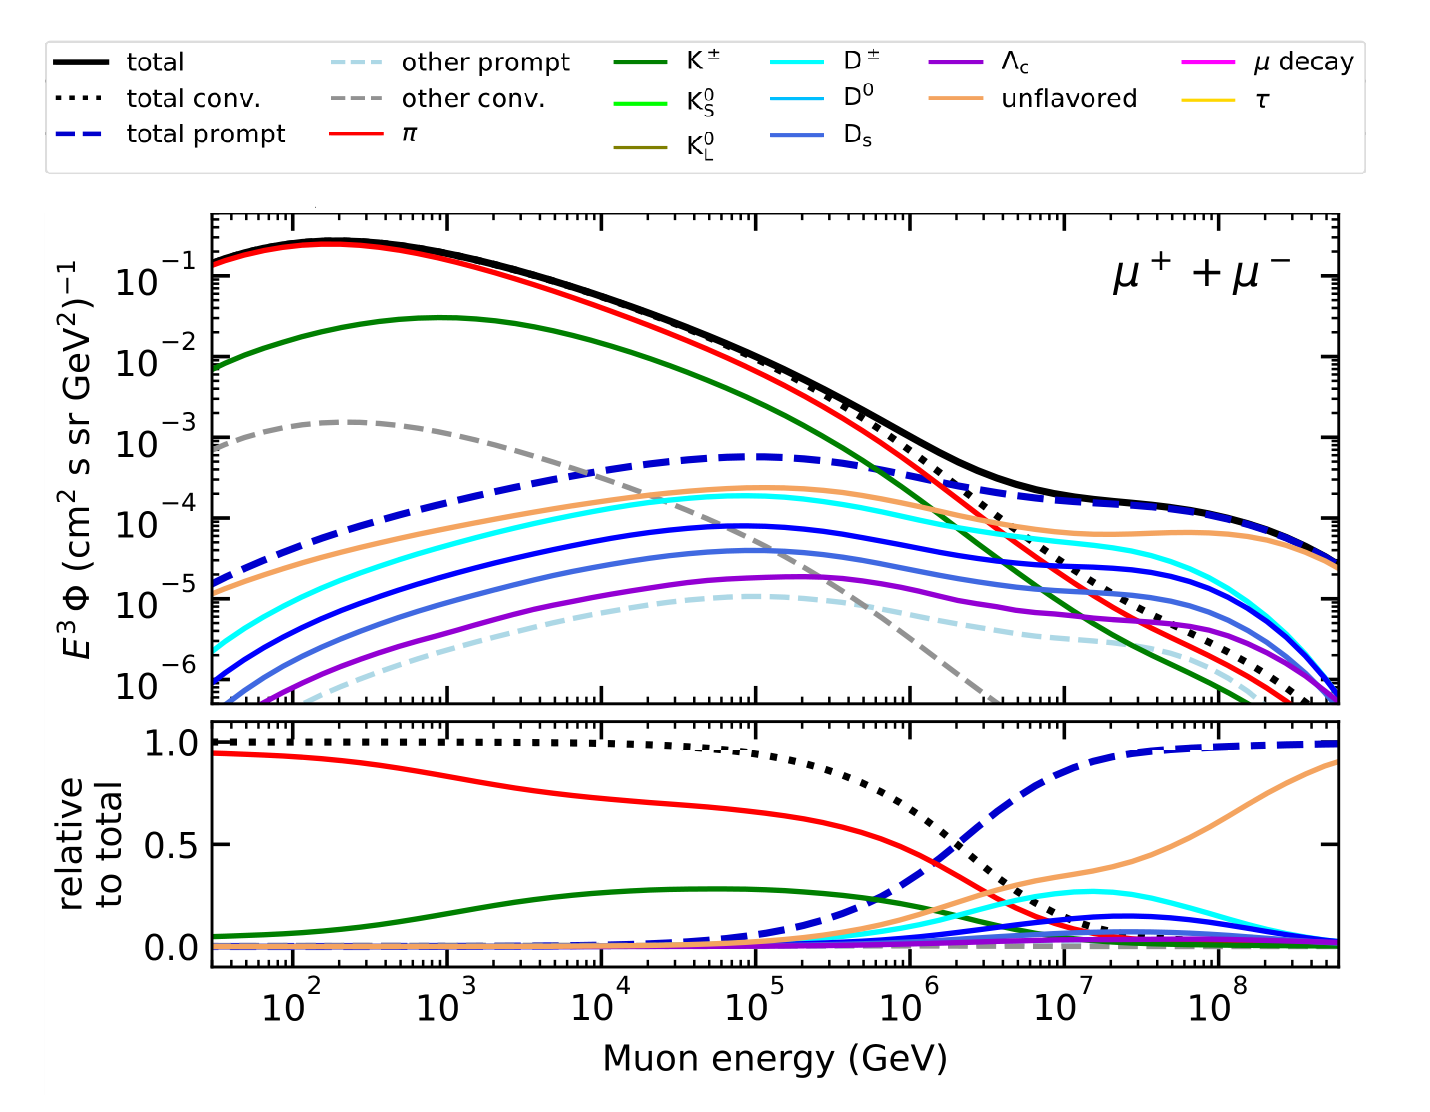
\includegraphics[width=0.8\textwidth]{muon_flux_fedynitch.png}
    \caption{Energiefluss atmosphärischer Myonen aufgeteilt nach den
     erzeugenden Hadronen, sowie deren relativen Beiträge,
      simuliert mit MCEq \cite{Fedynitch_2019}}
    \label{fig:prompt_muonflux}
\end{figure}

%%%%%%%%%%%%%%%%%%%%%%%%%%%%%%
% 2. Sektion plots und Reichweite
%%%%%%%%%%%%%%%%%%%%%%%%%%%%%%

% \newpage

% TODO heute
% 1: Warum Myonen:
%     - rel hohe Lebensdauer bei geringerer Wechselwirkungsrate 
%     -> hohe Reichweite

%     PLOT 
%     - Reichweite Plot aus Alexandrov

% 2: Myonen Spektrum

%   - Myonen auf sea level am häufigsten (alexandrov)
%     Zhang plot MYONEN RATE
    
%  todospäter 
%
% - wechselwirkungen (alexandrov)
%     - Wirkungsquerschnitt von röntgenstrahlung und Myonen vergleichen
% %
%   weiteres zu myonen spektrum: \\
%   
%   meiste myonen kommen aus vertikaler richtung

Auf Meereshöhe liegt die Flussdichte von Myonen typischerweise bei ca. 
$1 \; \frac{\mathrm{Myon}}{\mathrm{cm}^2 \; \mathrm{min}}$.  \cite{PDG2020} \cite{Schouten2019}

Da die Dichte des Erdreichs wesentlich höher ist als die der Atmosphäre,
nimmt die Myonenrate mit steigender Tiefe rapide ab,
wie in Abb. \ref{fig:Tiefenrate} zu sehen ist.

Die Reichweite kosmischer Myonen ist in Abb. \ref{fig:reichweite} zu sehen.

\begin{figure}[h]
    \centering
    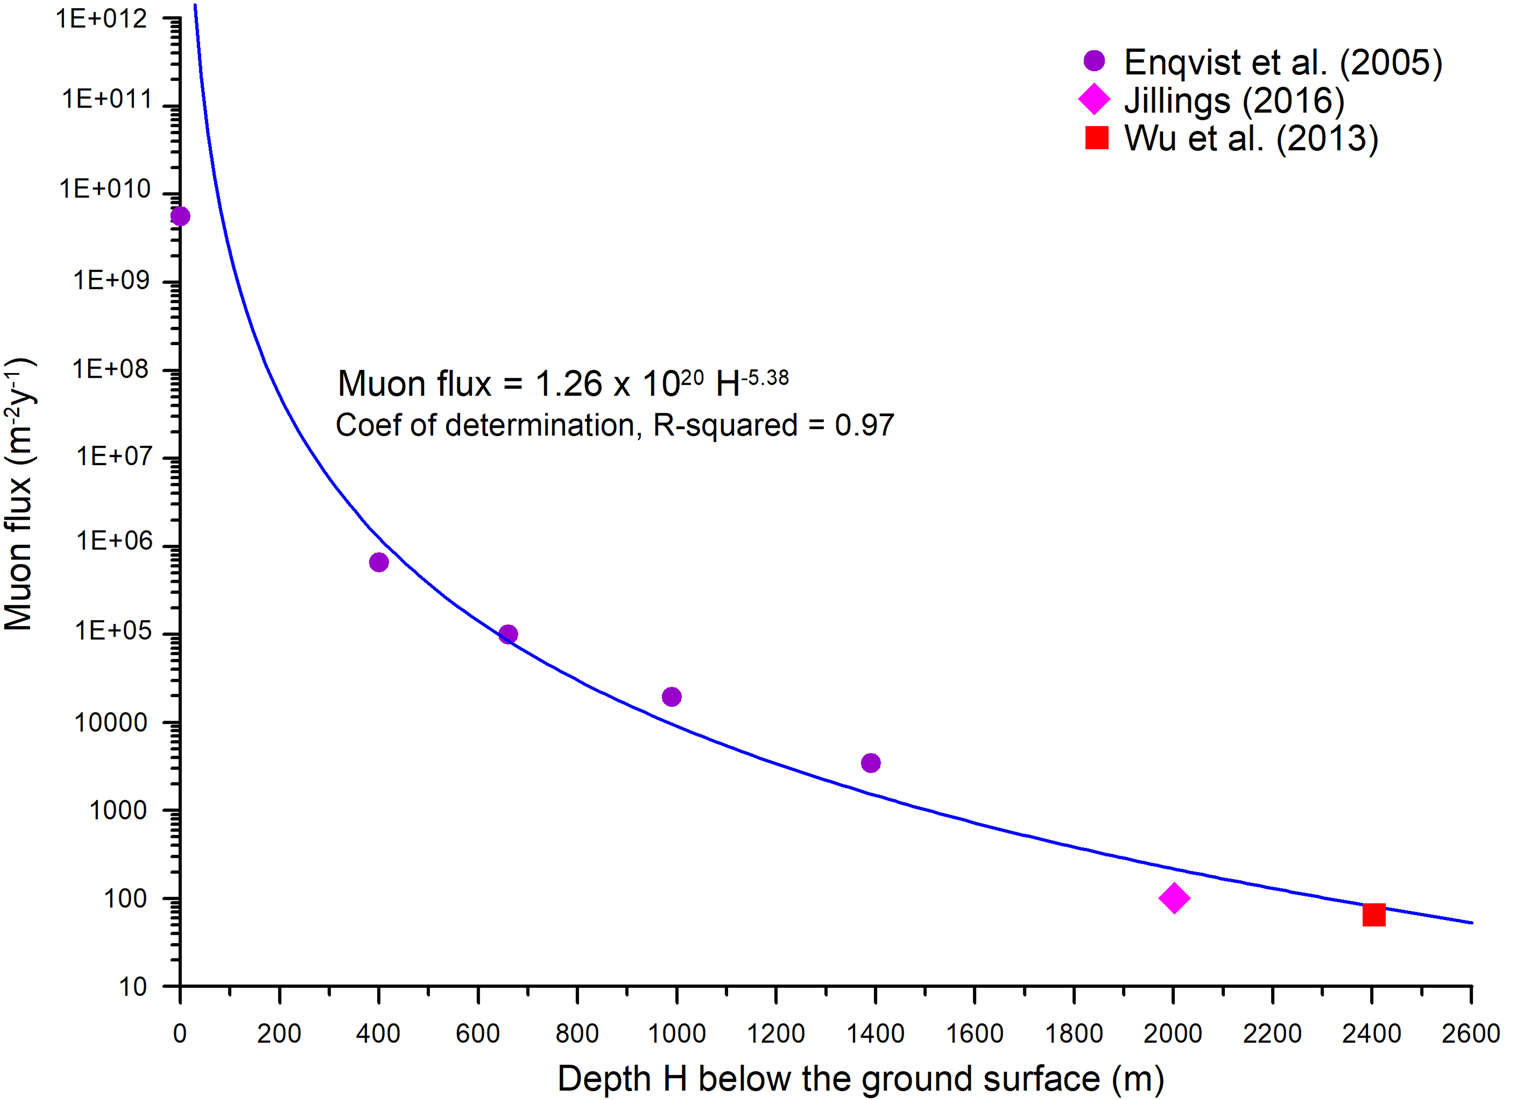
\includegraphics[width=0.7\textwidth]{Zhang_2020_muon_depth.png}
    \caption{
        Myonen Fluss gegen Tiefe unterhalb der Erdoberfläche.
        Mehrfarbig sind in verschiedenen Tiefen Messungen des Myonenflusses eingetragen.
        \cite{zhang2020}}
    \label{fig:Tiefenrate}
\end{figure}

\begin{figure}[h]
    \centering
    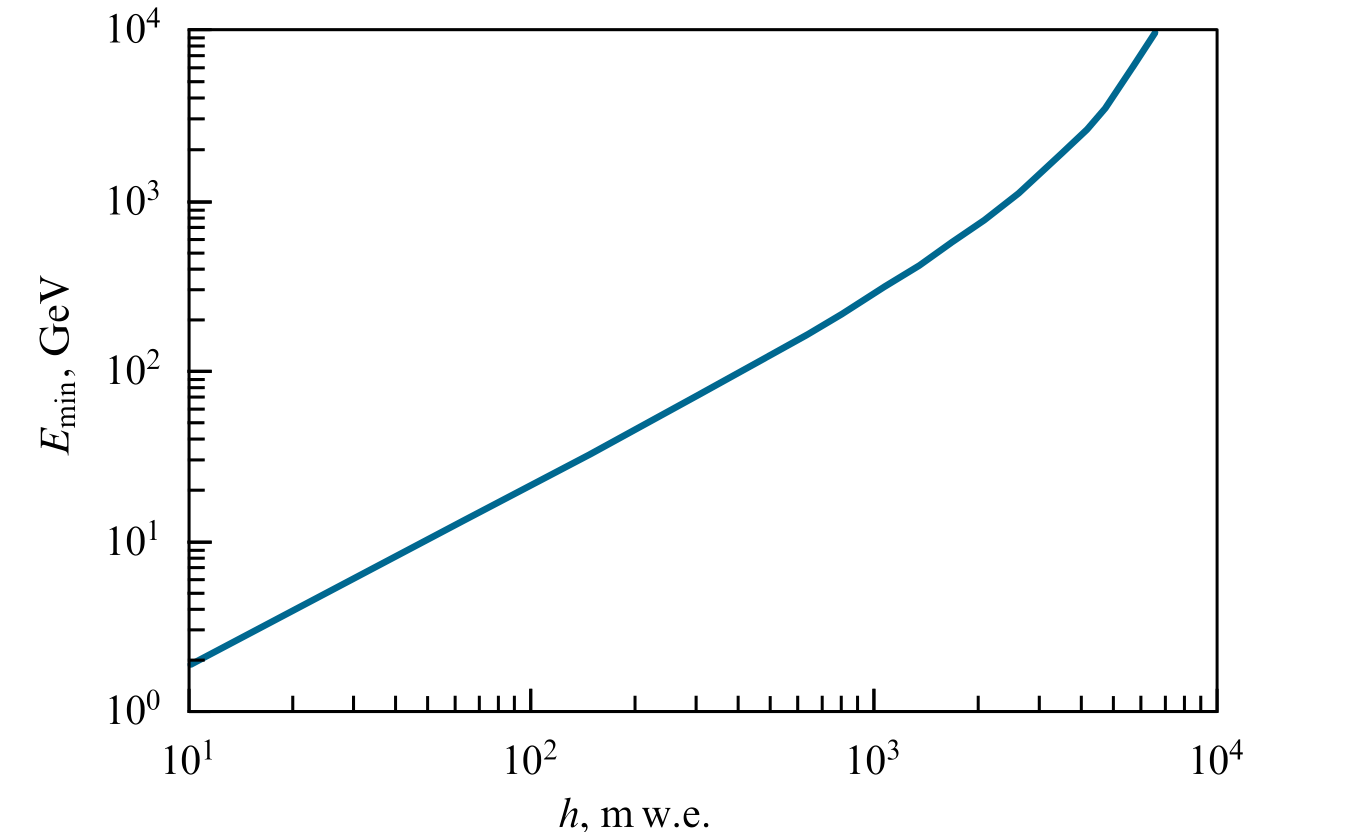
\includegraphics[width=0.7\textwidth]{reichweite.png}
    \caption{
        Die Reichweite von Myonen in $mwe$
        \cite{Alexandrov2017}}
    \label{fig:reichweite}
\end{figure}
\section{Myographie}

% Vergleich mit Röntgenaufnahme: 1. Myonen statt Röntgen-> höhere Reichweite
% Die Myographie ist eines in den Letzten Jahren immer mehr an Fahrt gewinnendes 
% Forschungsfeld. Da sie mit kosmischen Myonen funktioniert, erlaubt
% es ihr eine um Größenordnungen höhere Reichweite als z.B. die Röntgentomographie.

Die Myographie ist wie die Röntgentomografie, ein bildgebendes Verfahren.
Sie verwendet statt künstlich erzeugter Röntgenstrahlung bereits natürlich vorhandene kosmische Myonen.
Da Myonen einen wesentlich geringeren Wirkungsquerschnitt als Röntgen-Photonen
haben und teils sehr hohe Energien besitzen, haben sie eine wesentlich höhere Reichweite
als Röntgen-Photonen. Das ermöglicht der Myographie je nach 
angepeilter Präzision, Größe des Detektors und vorhandener Messzeit
eine Reichweite von mehreren Kilometern und ist daher
für weitläufige Untersuchungen größerer Strukturen oder des Erdreichs geeignet.
Es wurde z.B. zur Entdeckung noch unbekannter Kammern in der Cheops-Pyramide
verwendet\cite{pyramiden} oder zur Untersuchung des inneren eines Vulkans\cite{TANAKA2007104}.

% 1. Energieverlust und -ablenkung
Der Energieverlust und die Ablenkung der Myonen hängt von dem Bodenmaterial 
ab, durch das es propagiert.
Die Stärke des Energieverlusts ist proportional zur Dichte des 
Mediums für Energiebereiche der Myographie\footnote{Unter Vernachlässigung des LPM-Effektes bei hohen Energien.}.
Die Stärke der Ablenkung ist bei der Coulomb-Streuung zusätzlich zur 
Kernladungszahl $Z$ des Mediums proportional.
Im Rahmen der Energiebereiche und Distanzen der Myographie
liegt die mittlere Ablenkung bei $\sim \SI{1,5}{°}$ \cite{Alexandrov2017}.

% \marktodo{welche WW sind wie stark und wichtig? Plot aus dem Alexandrov!} 

% 2. Messzeit kann sehr lange werden
Da die Menge der atmosphärischen Myonen mit der Tiefe abnimmt, 
steigt benötigte Messzeit für präzise Messungen.
Die Messzeit lässt sich allerdings verkürzen durch Vergrößerung 
des Detektor Volumens

% 3. unterschied Detektor -> Winkel Auflösung ja/nein kein Bild standardmäßig
Genauso wie die Röntgentomografie einen Röntgenschirm braucht, der die Röntgenstrahlen 
"detektiert", verwendet die Myographie einen Teilchendetekor für Myonen.
Die einfachste Form eines Detektors für die Myographie zählt die Anzahl der Myonen die 
den Detektor pro Zeiteinheit durchqueren.
%  \marktodo{Vielleicht kurz erwähnen was für Arten von Detektoren möglich sind bzw. wie so eine detektion funktionieren kann.}
In Kombination mit der Messzeit lässt sich 
dann eine Rate angeben, wie viele Myonen pro Zeiteinheit durch den Detektor detektiert werden.

% Eine Vergrößerung ist allerdings nicht immer möglich aufgrund der Größe des Messraums
% und erhöht die Kosten des Projekts.

% Zusätzlich nimmt mit längeren Wegstrecken die Streuung der Myonen an den Atomen zu.
% Wenn der Detektor die Richtung der Myonen messen soll, wird diese also mit steigender Tiefe
% immer unschärfer.

% Die gemessene Rate $\frac{N_\mathrm{Myon}}{\mathrm{cm}^2 \; \mathrm{min}}$ 
% liefert erst eine Aussage, wenn\dots
% \marktodo{
%     ist die Reihenfolge des Erklärens sinnvoll? Sind das die wesentlichen Punkte um in die Myographie einzuleiten? \\\\
%     \marktodo{kleine ($\SI[]{\approx  1}[]{m^3}$) bis große ($\SI[]{< 1}[]{km^3}$) Strukturen untersuchbar.} 
%     \\
%     von JM:
%     Auch wenn es vermutlich in den nächsten Unterkapiteln noch ausführlicher erläutert wird, 
%     fehlt mir hier ein wenig der Grundgedanke, wie man denn jetzt genau Myographie verwenden 
%     kann. Du schreibst zwar explizit dass es "wie bei der Röntgenuntersuchung ist", 
% \\
%     aber vielleicht solltest du trotzdem erwähnen dass
%          mehr Masse pro Strecke = weniger Myonen ist,
%     und vielleicht auch erwähnen dass man 
%         mit einer Richtungsabhängigen Messung dann auch Profile erstellen kann.
% }

\textbf{Detektion eines Untergrundschachts mithilfe der Myographie} \\
%  \marktodo{anwendungsbeispiel vs experiment} 
Zur Veranschaulichung der Myographie wird im Folgenden ein Beispiel im Detail erklärt.
In \cite{Alexandrov2017} wird das  FIAN-SINP MSU Experiment beschrieben.
Ein Photo-Emulsions-Detektor hat über eine Messzeit von 4 Monaten   
Myonen richtungsabhängig gezählt.
Dieser wurde in einem Raum $\SI[]{30}[]{m}$ unterhalb der Erdoberfläche 
installiert. 
Der Versuchsaufbau ist in Abb. \ref{fig:alexandrov_messaufbau} zu sehen.

Ziel des Versuchs war es herauszufinden, ob der Aufzugsschacht in der Messung sichtbar ist. 
Parallel wurde eine Simulation der Messung zum Vergleich erstellt.
In Abb. \ref{fig:alexandrov_ergebnisse} sind die Ergebnisse zu sehen.
Der rote Kasten zeigt die Richtung des Aufzugsschachts.
Der rote Bereich innerhalb des Kastens bedeutet eine hohe Intensität an Myonen aus dieser Richtung.
Da in dem Schacht lediglich Luft ist, verlieren die Myonen beim Propagieren
durch die Luft wesentlich weniger Energie als im Erdreich, daher wurden aus dieser Richtung besonders viele Myonen detektiert.

Zusammenfassend konnte also erfolgreich mithilfe eines Photo-Emulsions-Detektors
 ein Untergrundschacht entdeckt bzw. gemessen werden.

\begin{figure}
    \centering
    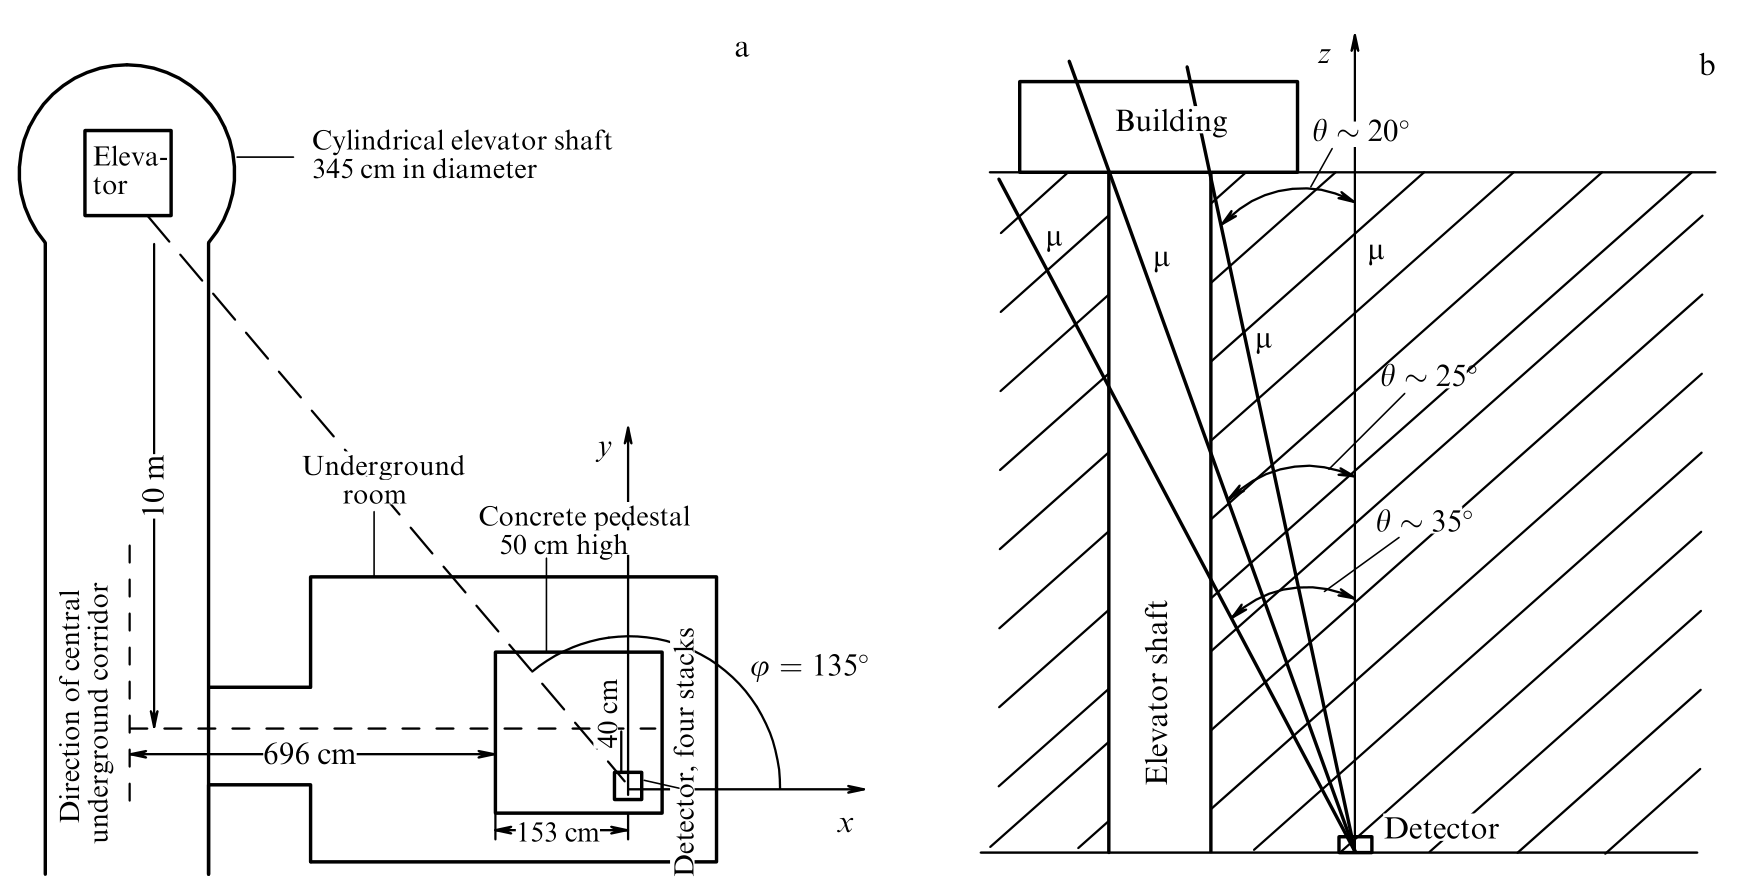
\includegraphics[width=0.9\textwidth]{alexandrov_messaufbau}
    \caption{Horizontale (a) and vertikale (b) Sicht auf das FIAN-SINP MSU Experiment \cite{Alexandrov2017}.
    Der Detektor hat in einer Tiefe von \SI[]{30}[]{m} über einen Zeitraum von 4 Monaten
    Myonen richtungsabhängig gemessen. Ziel war es, den Aufzugsschacht auflösen zu können.
    Die Anordnung der Koordinatenachsen ist im Detektorsystem angegeben.}
    \label{fig:alexandrov_messaufbau}
\end{figure}

\begin{figure}
    \centering
    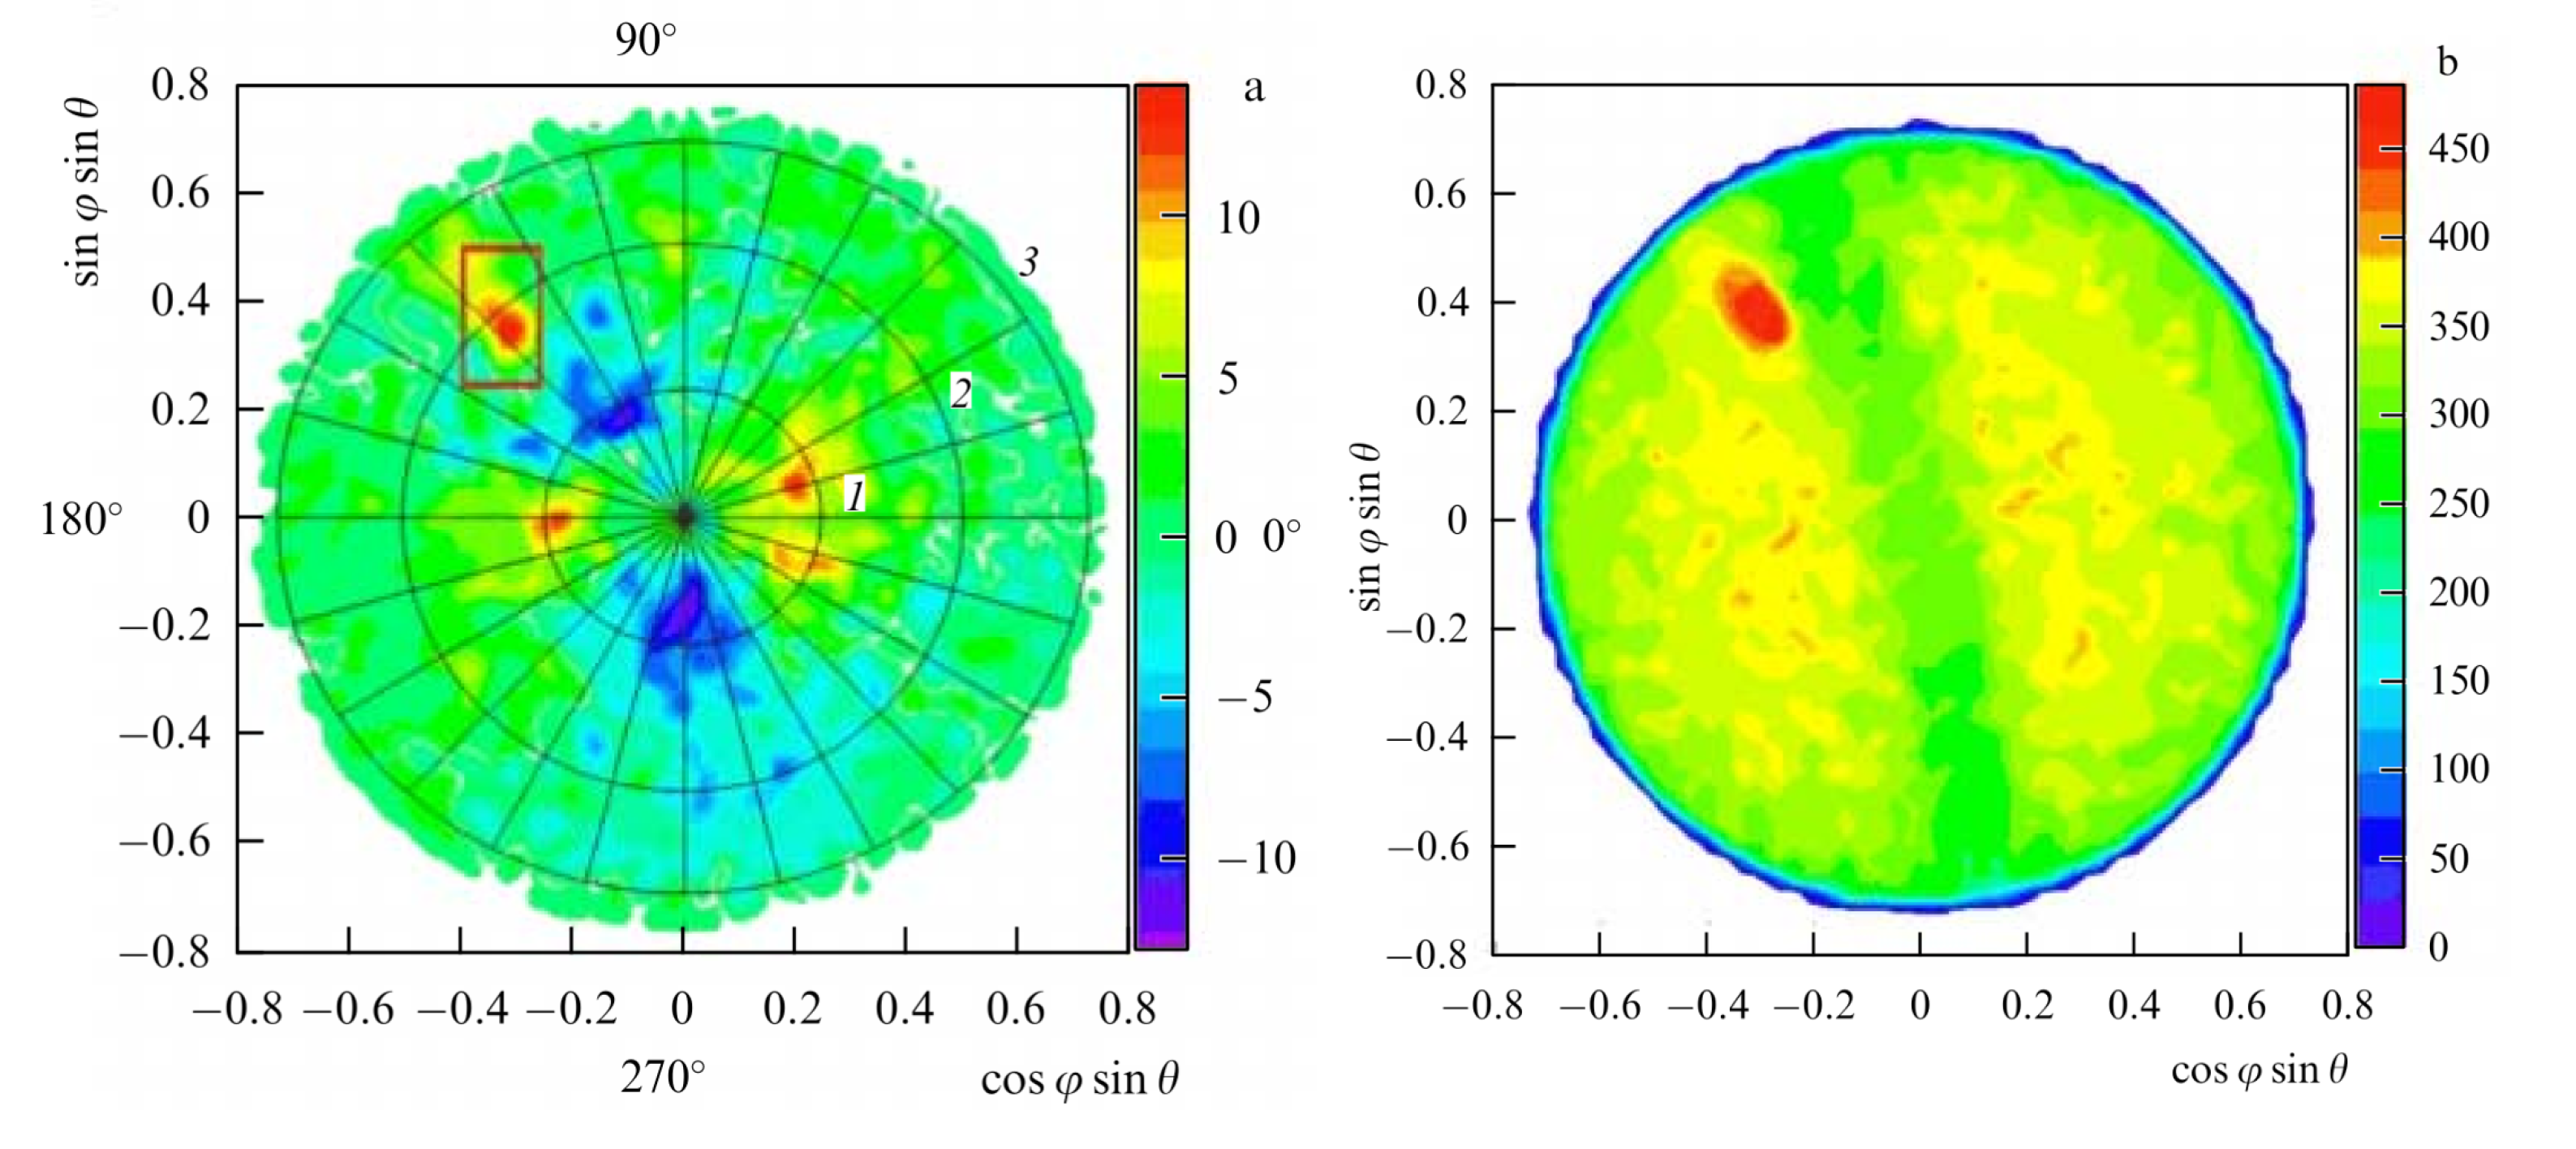
\includegraphics[width=0.93\textwidth]{alexandrov_beide}
    \caption{
        (a) Zweidimensionale Spurendichteverteilung der Myonen
        \SI[]{30}[]{m} unter der Erde. 
        Das rote Rechteck markiert den Blickwinkel in Richtung des Aufzugschachts. 
        Die Kreise nummeriert mit 1, 2 und 3, markieren jeweils die Zenitwinkel $\theta = 15°$, $30°$ und $45°$
        %
        (b) 
        Simulierte Verteilung aus der Simulation. Der deutlich zu erkennende rote Fleck
        repräsentiert einen hohen Myonenfluss aus der Richtung des Aufzugsschachts.
        Die Verteilungen der Spurendichte sind in Form der Variablen $\sin \phi \sin \theta$ 
        und $\cos \phi \sin \theta$ dargestellt. Sie repräsentieren den Einfallswinkel der detektierten Myonen
        gegenüber der Senkrechten zur Detektorebene.
        \cite{Alexandrov2017}
    }
    \label{fig:alexandrov_ergebnisse}
\end{figure}

% - $\frac{I_{det}}{I_0} \sim \sum m$
%   Myonen Abschwächung gegenüber Oberfläche ist proportional zur Masse des 
% durchquerten Materials


% - Detektoren messen Myonen-Intensität (N, E, $\phi$)
%     - Erkenntnisse über Beschaffenheit des Masse “über” einem
% - anhand eines Beispiels:
% - Man ist in einer erforschten Pyramide und möchte herausfinden ob es noch unentdeckte Hohlräume gibt.
% - $\rho * V = m$
%     - Myographie liefer die die Masse quasi, denn je mehr masse durchquert wird desto mehr Energie verlieren die Myonen und zerfallen
%     - man gibt der Myographie noch V und bekommt so rho des materials → Eigenschaften des gemessens Materials
% - Einordung der myographie
%     - strahlungsquelle und intensität immer vorhanden und bekannt
% - Detekoren auch ohne Strom betreibbar
% - viele Anwendungsfelder
% - unterscheidung zwischen myographie und myon tomographie
\chapter{Verwendete Myonen Simulationssoftware}

Dieser Abschnitt führt die Myonen Simulationssoftwares,
EcoMug und PROPOSAL ein.

\section{Myonen Erzeugung mit EcoMug}

% EcoMug ist eine reine C++11-Header-Bibliothek 
% zur Erzeugung von Myonen aus kosmischer Strahlung 
% (CR), die auf einer Parametrisierung experimenteller 
% Daten basiert. Im Gegensatz zu anderen Werkzeugen 
% bietet EcoMug die Möglichkeit, aus verschiedenen Oberflächen 
% (Ebene, Zylinder und Halbkugel) zu erzeugen, wobei die 
% korrekte  der erzeugten Spuren 
% erhalten bleibt. EcoMug ermöglicht auch die Erzeugung von 
% CR-Myonen nach benutzerdefinierten Parametrisierungen ihres 
% differentiellen Flusses.

EcoMug\footnote{\url{https://github.com/dr4kan/EcoMug}} ist ein C++-Programm 
zur Generierung einzelner Myonen \cite{EcoMug} anhand einer
Parametrisierung des differentiellen Myonenflusses. 

Es lässt sich neben dem standardmäßig implementierten Myonenfluss
auch ein eigener definieren.
Außerdem bietet EcoMug die Möglichkeit, Myonen aus verschiedenen Oberflächen (Ebene, Zylinder und Halbkugel) mit physikalisch korrekter
Winkel- und Impulsverteilung zu erzeugen. 
Zu guter Letzt ist EcoMug mit besonderem Merkmal auf Schnelligkeit entwickelt worden.



\section{Lepton Propagation mit PROPOSAL}

PROPOSAL\footnote{\url{https://github.com/tudo-astroparticlephysics/PROPOSAL}} ist ein in C++ geschriebenes Simulationsprogramm und steht für 
\textbf{Pr}opagator with \textbf{O}ptimal \textbf{P}recision 
and \textbf{O}ptimized \textbf{S}peed for \textbf{A}ll \textbf{L}eptons. 
\cite{proposal, proposal2, proposal3}
%  nahe dem geografischen Südpol in der Antarktis.
Über den Monte-Carlo-Algorithmus lassen sich Leptonen wie
Elektronen, Myonen und Taus durch verschiedene Medien propagieren. 
% Propagieren bedeutet, dass die Wechselwirkungen des Teilchens mit
% der Materie durch das es fliegt simuliert wird.
PROPOSAL kann den Energieverlust, Ablenkung sowie Zerfall der Teilchen simulieren.
% Bei Zusammenstößen mit Materie verliert es Energie und ändert seine Richtung.

PROPOSAL wird hauptsächlich an der TU Dortmund weiterentwickelt 
sowie als OpenSource Projekt auf GitHub. 
Es ist unter anderem ein Bestandteil der Simulationskette des Neutrino-Detektors IceCube \cite{icecube}.
Im Vergleich dazu sei auch das Simulationsprogramm GEANT4 erwähnt, welches speziell
für die Simulation von Teilchen innerhalb eines Detektors konzipiert ist.
PROPOSAL ist dahingehend optimiert, über längere Strecken ($> \SI[]{1}[]{km}$) Teilchen 
zu propagieren, daher ist es auch für die Anwendung in der Myographie
gut geeignet.

\subsection{Funktionsweise von PROPOSAL}
\label{sec:pp-theorie}

In PROPOSAL sind für die Propagation von Myonen die Wirkungsquerschnitte für 
Ionisation, Bremsstrahlung, Paarproduktion und Photonukleare Wechselwirkung 
implementiert. Außerdem wird der Zerfall anhand der Lebensdauer simuliert. \cite{proposal}
In Abb. \ref{fig:energieverlust_pp} ist der mittlere Energieverlust
der verschiedenen Wechselwirkungen dargestellt.

Die meisten\footnote{Nicht stochastisch bspw.: 
die Dichtekorrektur bei der Ionisation. Sie ist ein rein kontinuierlicher Prozess} 
physikalische Wechselwirkungen sind stochastisch, das heißt
Teilchen verlieren in diskreten Interaktionen Energie bzw. werden abgelenkt.
Die Anzahl an Bremsstrahlungswechselwirkungen divergieren allerdings für 
immer kleinere Energien gegen unendlich, was bedeuten würde, dass unendlich 
viele Interaktionen berechnet werden müssten. 
Aufgrund dieses Problems und um die Präzision zugunsten der Laufzeit steuern
zu können, gibt es einen frei wählbaren Energieschnitt (Energy-Cut).

\begin{figure}[]
    \centering
    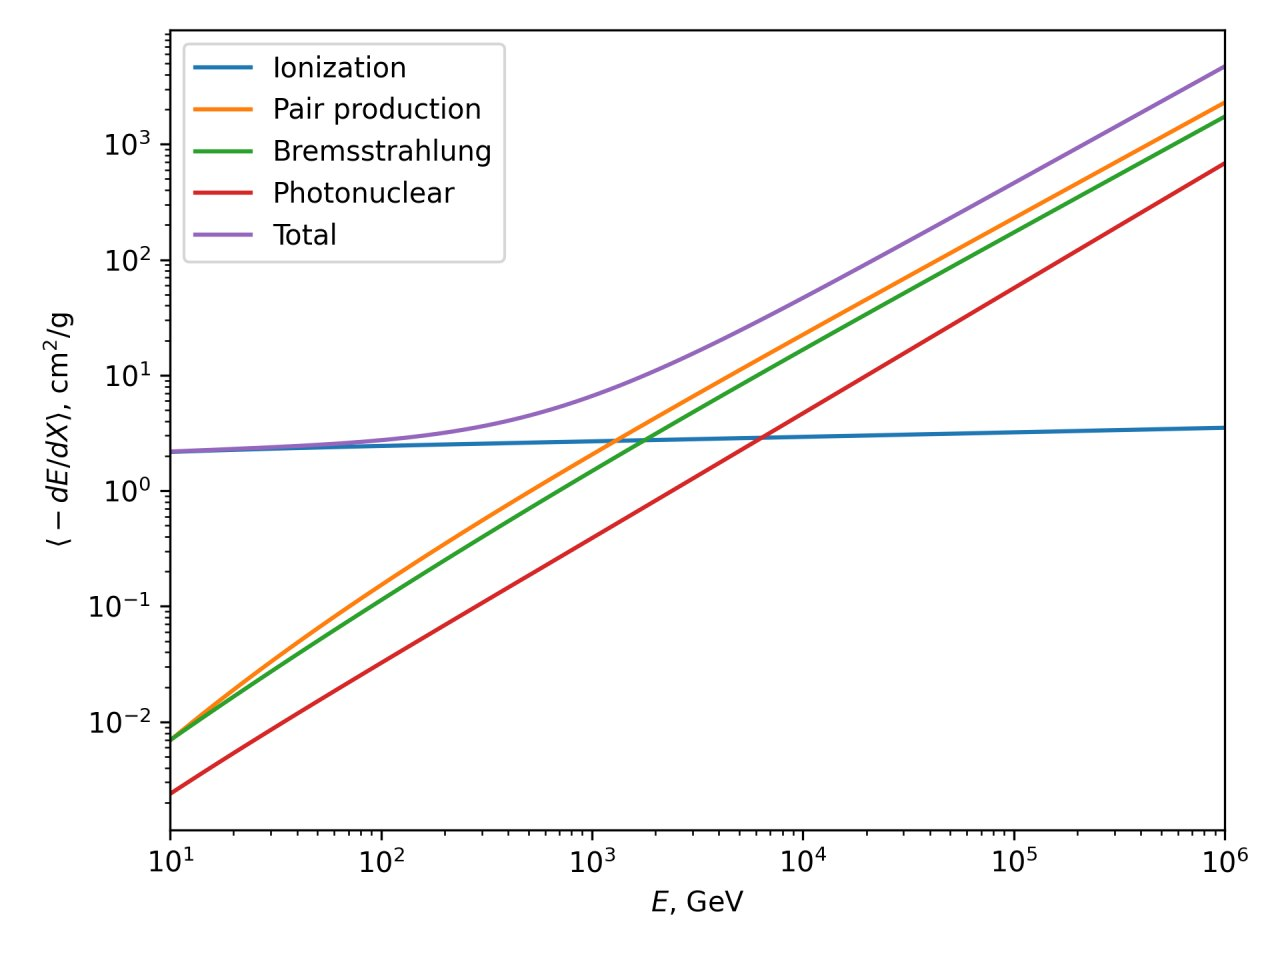
\includegraphics[width=0.55\textwidth]{wechselwirkungen PP.jpg}
    \caption{Der mittleren Energieverlust von Myonen in Standardgestein. Mit PROPOSAL simuliert.}
    \label{fig:energieverlust_pp}
\end{figure}

Der Energy-Cut ist als absoluter $E_\mathrm{cut}$ bzw. relativer $v_\mathrm{cut}$ konfigurierbar.
Unterhalb des Energieschnitts werden die Interaktionen statt stochastisch zufällig gezogen zu werden,
kontinuierlich berechnet.
Das bedeutet, dass ein durchschnittliches $\frac{\mathrm{d}E}{\mathrm{d}x}$
für die kontinuierlichen Energieverluste berechnet wird. 
Dadurch werden die sonst unendlichen Interaktionen der Bremsstrahlung endlich und so simulierbar.
%  \marktodo{warum ist die kont rand wichtig?} 
Es lässt sich optional die sog. kontinuierliche Randomisierung
aktivieren, welche die kontinuierlichen Berechnung über eine Gauß-Verteilung stochastisch verschmiert.
% Die Vielfachstreuung lässt sich optional aktivieren, wobei 3 Parametrisierungen mit 
% unterschiedlichen Approximationen implementiert sind. 
% Davon ist Molière die genauste Implementierung, dann kommt HighlandIntegral als Gaußsche Näherung
% der Molière Parametrisierung. Danach kommt Highland, welches HighlandIntegral ist mit der Annahme, dass 
% die Teilchenenergie während eines Propagationschritts konstant bleibt. 

PROPOSAL wird die Energie, Position, Richtung und Art des zu propagierenden Teilchens 
sowie Sektoren für die Propagation übergeben.
Diese Sektoren werden über eine Liste an implementierten Medien 
und selbst konfigurierbaren Dichte-Verteilungen definiert.
Pro Sektor lässt sich ein individueller Energy-Cut setzen.
Es sind verschiedene Medien wie z. B. Standardgestein oder Wasser implementiert. 
Zudem kann bestimmt werden, wann die Propagation gestoppt werden soll: 
Bis zu einer Energie, nach einer bestimmten Strecke oder 
nach Verlassen eines Sektors.
Zudem muss ein $E_\mathrm{cut}$ bzw. $v_\mathrm{cut}$ gesetzt werden. 
Als Ausgabe übergibt PROPOSAL dem Nutzer ein Objekt \textit{track}, welches 
Informationen über die Propagation des Teilchens innehält.
Es sind unteranderem Endposition, Endenergie und propagierte Strecke abrufbar.  

%  \marktodo{größenordung für vcut und laufzeiten angeben.} 

Genauere Informationen über die Funktionsweise von PROPOSAL lassen sich
aus den Veröffentlichungen \cite{proposal}, \cite{proposal2} und \cite{proposal3} nachlesen.
    

% PROPOSAL hat zwei verschiedene Arten von Tabellen. Einmal die Tabellen für Wirkungsquerschnitte. 
% Da gibt es die Tabellen die dNdx interpolieren. Diese Tabellen sind zweidimensional (in E und v), 
% und das sind deshalb die Tabellen die lange zum bauen brauchen.

% Die anderen Tabellen sind die Tabellen für die “PropagationUtilities”, dessen Stützstellen 
% mit dieser Einstellung verändert werden. Diese werden genutzt, um zum Beispiel die 
% Integralgleichungen zu lösen. Diese Tabellen sind jedoch alle eindimensonal, 
% außerdem basieren sie auf den Interpolationstabllen für die Wirkungsquerschnitte. 
% Deshalb sind die relativ schnell zu bauen.
% \chapter{Vorbereitung und Konfiguration der Simulationskette}
% \chapter{Simulation eines Detektors in verschiedenen Wassertiefen}
\chapter{Simulation eines Detektors unter verschiedenen Wassertiefen}

%Einleitung was hier passiert

Aufgrund der Bergbauvergangenheit sind im Ruhrgebiet viele Bohrungen gemacht worden.
In einige der Bohrungen ist ein Metallrohr mit einem Durchmesser von \SI[]{10}[]{m} 
eingelassen.
Um den Wasserstand der trocken gelegten Schichten zu überwachen
ist die Idee dieser Arbeit in eines dieser Rohre einen zylinderförmigen Detektor 
herunterzulassen und zu ermitteln welche Detektorraten erwartet werden.

Um zu ermitteln in welchen Rahmen der Wasserstand dieser Schichten messbar ist,
wird für den zylinderförmiger Detektor eine Grundfläche von 
\SI[]{75}[]{cm^2} angenommen. Er soll sich auf dem Boden der Bohrung befinden.
Es wird anhand des Schichtverzeichnisses der Bohrung ein Bodenmodell erstellt,
welches die unterschiedlichen Bodenzusammensetzungen über Variationen der
\textit{Standardrock}-Dichte.
Dieses ist die Basis für die Propagation mit PROPOSAL.
Kosmische Myonen werden mithilfe einer Parametrisierung des Myonenflusses auf Meereshöhe
mit EcoMug erzeugt.

% todospäter
% \marktodo{veranschaulichung des messaufbaus: Luft, Boden, Wasser Detektor???} 

% Die Simulation besteht im Wesentlichen aus zwei Teilen. 
% Als Erstes werden Myonen aus einer Parametrisierung 
% des Myonenflusses auf Meereshöhe mit EcoMug gezogen und zwischengespeichert.
% Diese Myonen werden dann von PP durch das Bodenmodell bis zu dem Detektor propagiert. 
% Als Ergebnis liefert PROPOSAL, wie viele Myonen am Detektor angekommen sind.
% Die entsprechende Detekorzählrate wird im Kapitel Ergebnisse errechnet.




\section{Bodenmodell}
\label{sec:bodenmodell}
%%%%%%%%%%%%%%%%%%%%%%%%%%%%%%%%%%%%%%%%%%%%%%%%%%%%%%%%%%
% bohrung eckdaten, grundlage
%%%%%%%%%%%%%%%%%%%%%%%%%%%%%%%%%%%%%%%%%%%%%%%%%%%%%%%%%%
\subsection{Beschreibung der Bohrung}
Als Basis für das Bodenmodell dient eine Bohrung in der 
Kirchheller Heide\footnote{
    \url{boreholemap.bgr.de/mapapps/resources/apps/boreholemap/} 
    Standort: (351221,19 5719599,6) 
    ID: DABO\_65808 nahe dem Schwarze Heide Airport},
welches freundlicherweise von 
Prof. Dr. Ing. Tobias Rudolph\footnote{Technische Hochschule Georg Agricola - Forschungszentrum Nachbergbau}
zur Verfügung gestellt wurde.
In Abb. \ref{fig:Schichtverzeichnis_auszug} ist ein Ausschnitt des Schichtverzeichnis der Bohrung zu sehen.
Das vollständige Schichtverzeichnis befindet sich im Anhang
\ref{fig:Schichtverzeichnis_komplett}

\begin{figure}[h]
    \centering
    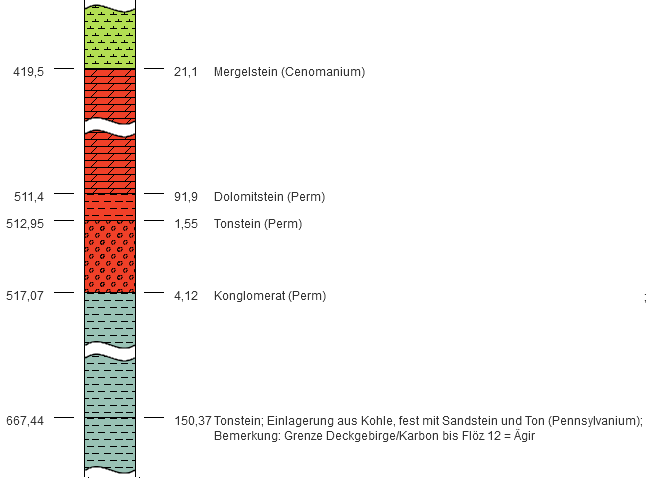
\includegraphics[width=0.97\textwidth]{schichtverzeichnis_auszug.png}
    \caption{Ein Auszug aus einer Bohrung in der Kirchheller Heide 
    Die Tiefe in Metern (links) ist als das untere Ende der Schicht gemeint,
    d.h. die Dolomit-Schicht geht von 419,5 bis 511 Metern.
    Die rechte Zahl ist die Höhe der Schicht in Metern.
    Hinter der Bodenart ist die jeweilige erdgeschichtliche Epoche in Klammern.
    Das vollständige Verzeichnis ist im Anhang \ref{sec:alle_schichten} zu sehen.}
    \label{fig:Schichtverzeichnis_auszug}
\end{figure}
 
Die Schichten von \num{1259} bis \SI{419,5}{m} (siehe Abb. \ref{fig:Schichtverzeichnis_auszug})
wurden aufgrund des Bergbaus in der Region trocken gelegt und während der Benutzung trocken gehalten 
(im folgenden \textit{Wasser-Schichten genannt}).
Jene Schichten haben ein sog. Hohlraumvolumen von ca. \num{5} bis \SI{15}{\percent}
welche naturgemäß mit Wasser gefüllt sind.
Das Hohlraumvolumen entspricht im Allgemeinen dem das, was von Kristallen 
in einer dichtesten Kugelpackung erwartet wird.
Zusätzlich zu dem Hohlraumvolumen müssen Risse berücksichtigt werden, welche zusätzlich 
\num{5} bis \SI{10}{\%} an Volumen ausmachen können und sich ebenfalls mit Wasser
füllen können.

Die Geschwindigkeit des Wasseranstiegs liegt in Größenordnungen von 
\SI{10}{cm} pro Woche. 

%%%%%%%%%%%%%%%%%%%%%%%%%%%%%%%%%%%%%%%%%%%%%%%%%%%%%%%%%%
%  modell erstellen
%%%%%%%%%%%%%%%%%%%%%%%%%%%%%%%%%%%%%%%%%%%%%%%%%%%%%%%%%%
\subsection{Umsetzung des Bodenmodells}
% Ziel ist es bei verschiedenen Wasserständen innerhalb der 
% entsprechenden Schichten die Detektorrate zu simulieren.
Es wird nun ein Bodenmodell anhand der Bohrung erstellt.

Zunächst wird festgestellt, dass die einzelnen Schichten jeweils aus einer 
Zusammensetzung verschiedener Gesteinsarten bestehen.
Da in PROPOSAL nicht die Möglichkeit besteht beliebige Gesteine
in ihrer chemischen Zusammensetzung zu modellieren, werden die Schichten mit 
dem Medium 
\textit{Standardrock}\footnote{Mit \textit{Standardrock} ist ein Material mit $Z = 11$, $A = 22$ und einer Dichte
von $\rho = \SI{2.65}[]{g/cm^3}$ gemeint \cite{Chirkin2015}.}
genähert.
Die Dichten werden entsprechend der echten Medien gesetzt.
Als Dichte der Schichten wird der Mittelwert zwischen $\rho_\mathrm{min}$
und $\rho_\mathrm{max}$ der jeweiligen 
Gesteinsarten\footnote{
    Tonstein, Dolomitstein, Sandstein: \cite{JS},
    Kalkstein \cite{RC},
    Mergelstein \cite{VNK},
    Sand \url{hausjournal.net/dichte-sand}}
benutzt (siehe Tabelle \ref{tab:gesteinarten})
In Abb. \ref{fig:dichte_modell} ist das Bodenmodell als Plot gegen die Tiefe abgebildet.

\begin{table}[h]
    \caption{Benutzte Dichten der verschiedenen Gesteinsarten in [\si[]{g/cm^3}].
    KS steht für Kalkstein, TS für Tonstein.}
    \centering\begin{tabular}{c c c c}
        Gesteinsart & $\rho_\mathrm{min}$ & $\rho_\mathrm{max} $ & $\rho_\mathrm{avg}$ \\
        \toprule
        Sand & 1,43 & 1,47&1,45 \\
        Tonmergelstein (\SI[]{20}[]{\%} KS, \SI[]{80}[]{\%} TS)&&&1,87 \\
        Kalkmergelstein (\SI[]{70}[]{\%} KS, \SI[]{30}[]{\%} TS)&&&2,045 \\
        Kalkstein  & 1,55 & 2,75 & 2,15 \\
        Mergelstein & 1,2 & 3 & 2,1 \\
        Dolomitstein & 2,4 & 2,9 & 2,65 \\
        Tonstein & 1,3 & 2,3 & 1,8 \\
        Sandstein & 2 & 2,8 & 2,4 \\
        % Konglomerat\footnote{\url{steine-und-minerale.de/atlas.php?f=3&l=K&name=Konglomerat}} & 2,3 & 2,6 & 2,45 \\
    \end{tabular}
    \label{tab:gesteinarten}
\end{table} 

%  \marktodo{rausgeschmissen sinnvoll?} 
% Des Weiteren sind einige Schichten unter
% \SI[]{1}[]{m}  \marktodo{wo mache ich die grenze?}
% Da so kleine Schichten im Anbetracht der bereits gemachten Näherungen
% keinen Mehrwert an Genauigkeit liefern, werden jene ignoriert.
% Die freie Lücke wird mit der darüber liegenden Schicht aufgefüllt.

\begin{figure}[h]
    \centering
    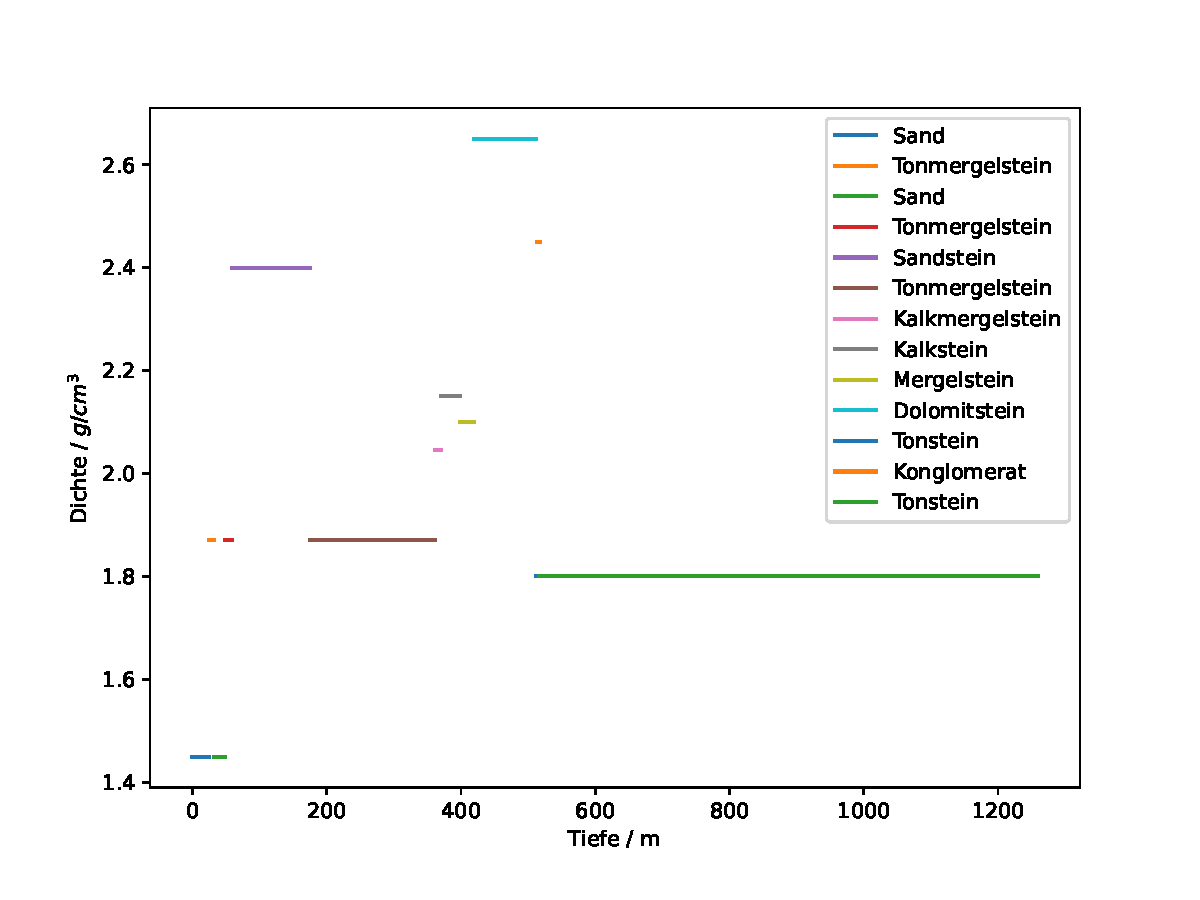
\includegraphics[width=\textwidth]{geology_modell_full.pdf}
    \caption{Das Bodenmodell nach Dichte und Tiefe aufgelöst.
    Der Tonstein in grün rechts, 
    sowie die Dolomitschicht oben in hellblau, können mit Wasser vollaufen.}
    \label{fig:dichte_modell}
\end{figure}

% wie wird volllaufen mit wasser modelliert.
Zur Modellierung der Wasser-Schichten,
wird angenommen, dass die Dichte 
einer Wasser-Schicht, das Gestein mit einem
Hohlraumvolumen von \SI[]{10}[]{\%} repräsentiert. 
Es wird also für Wasser-Schichten $\rho_\mathrm{Gestein10\%} == \rho_\mathrm{avg}$ angenommen.
Im trockenem Zustand wird der Hohlraum mit einer Luftdichte von 
$\rho_\mathrm{Luft} = \SI[]{0}[]{g/cm^3}$ genähert.
Daraus folgt 
\begin{equation}
    \rho_\mathrm{Gestein0\%} = \rho_\mathrm{Gestein10\%} / \num[]{0,9}.
\end{equation}
Mit $\rho_\mathrm{Gestein0\%}$ als die Dichte des Gesteins ohne Hohlraumvolumen.
Wenn ein Gestein mit Wasser vollläuft, wird die neue Dichte $\rho_\mathrm{nass}$ über
\begin{equation}
    \rho_\mathrm{nass} = 0,9*\rho_\mathrm{Gestein0\%} + 0,1*\rho_\mathrm{Wasser}
\end{equation}
berechnet. Für die Dichte des Wasser $\rho_\mathrm{Wasser}$ wird 
$\SI[]{1.0}[]{g/cm^3}$ \cite{Patterson_1994} angenommen.

Für die Tonstein-Schichten bspw. mit $\rho = \SI[]{1,8}[]{g/cm^3}$ 
steigt die Gesamtdichte mit Wasser auf \SI[]{1,9}[]{g/cm^3}.
Also eine effektive Erhöhung um ca. \SI[]{5,5}[]{\%}.



% \section{Konfiguration von EcoMug}
\section{Myonenfluss}
\label{sec:myonenfluss}
%%%%%%%%%%%%%%%%%%%%%%%%%%%%%%%%%%%%%%%%%%%%%%%%%
% gaisser param
%%%%%%%%%%%%%%%%%%%%%%%%%%%%%%%%%%%%%%%%%%%%%%%%%

Zur Beschreibung des Myonenflusses auf der Erde wird die 
\textit{Gaisser}-Parametrisierung \cite{Alexandrov2017} verwendet:
\begin{equation}
        \frac{\mathrm{d}N_{\mu}}{\mathrm{d}E_{\mu}\mathrm{d}\Omega} \approx \frac{0.14 E_{\mu}^{-2.7}}{\text{GeV cm$^2$ s sr}} \left(\frac{1}{1+1.1 E_{\mu}\cos \theta / (115 \text{GeV})} 
        + \frac{0.054}{1+1.1 E_{\mu}\cos \theta / (850 \text{GeV})}\right).
    \label{eqn:dN_dE}
\end{equation}

% \begin{equation}
    %     \begin{split}
        %     \frac{\mathrm{d}N_{\mu}}{\mathrm{d}E_{\mu}\mathrm{d}\Omega} &\approx \frac{0.14 E_{\mu}^{-2.7}}{\text{GeV cm$^2$ s sr}} \left(\frac{1}{1+1.1 E_{\mu}\cos \theta / (115 \text{GeV})} \\\
        %      &+ \frac{0.054}{1+1.1 E_{\mu}\cos \theta / (850 \text{GeV})}\right)
        %     \end{split} 
        % \end{equation}
        
        % \begin{multline}
%     d^2 = a^2 + b^2 + c^2 \geq a^2 + b^2 = a^2 + b^2 + 2ab - 2ab = (a+b)^2 - 2ab \\\ \geq -2ab
% \end{multline} 

% \begin{multline}
%     \frac{\mathrm{d}N_{\mu}}{\mathrm{d}E_{\mu}\mathrm{d}\Omega} \approx \frac{0.14 E_{\mu}^{-2.7}}{\text{GeV cm$^2$ s sr}} \left(\frac{1}{1+1.1 E_{\mu}\cos \theta / (115 \text{GeV})} \\\ + \frac{0.054}{1+1.1 E_{\mu}\cos \theta / (850 \text{GeV})}\right)
% \end{multline} 
    
% \label{eqn:dN_dE}
$N_{\mu}$ ist die Anzahl an Myonen, $E_{\mu}$ die Myonen Energie 
und $\Omega$ der Raumwinkel. Die Parametrisierung modelliert den Myonenfluss auf Meereshöhe.

Die zwei Terme in Klammern repräsentieren
jeweils die Beiträge über Zerfälle von Pionen bzw. Kaonen, wie beschrieben in Kap. \ref{sec:theorie}.
Die Parametrisierung gilt unter zwei Annahmen. Es wird die Krümmung der Erde vernachlässigt, 
welche den Zenit-Winkel einschränkt. Des Weiteren wird der Myon Zerfall vernachlässigt.
Folgende Einschränkungen gelten:
\begin{align}
    \theta < 70° \;\; \mathrm{und} \;\; E_\mu > \frac{\SI[]{100}[]{GeV}}{\cos \theta}.
\end{align}
Zur Vereinfachung wird angenommen dass das Bohrloch auf Meereshöhe beginnt. 
%  \marktodo{im EcoMug paper nachgucken welche einschränkungen deren parametrisierung hat} 
% Die Myo
% Die ursprüngliche Energien der Myonen die am Detektor ankommen im Kontext dieser Arbeit,
% liegen weit über $\SI[]{100}[]{GeV}$ daher ist die zweite Bedingung auch erfüllt.

Zur Einhaltung dieser wird in EcoMug das Maximum für den Winkel $\theta$ auf $30°$ konfiguriert.
Da die Myonen mehr als \SI[]{600}[]{GeV} benötigen um den Detektor zu erreichen,
ist die Zweite Bedingung auch erfüllt.
Es wird für die Erzeugung der Myonen mit EcoMug der Energiebereich von \SI[]{600}[]{GeV} bis 
\SI[]{200}[]{TeV} gewählt.
In Abb. \ref{fig:ecomugplot} ist das verwendete Energiespektrum aus EcoMug zu sehen.

\begin{figure}[]
    \centering
    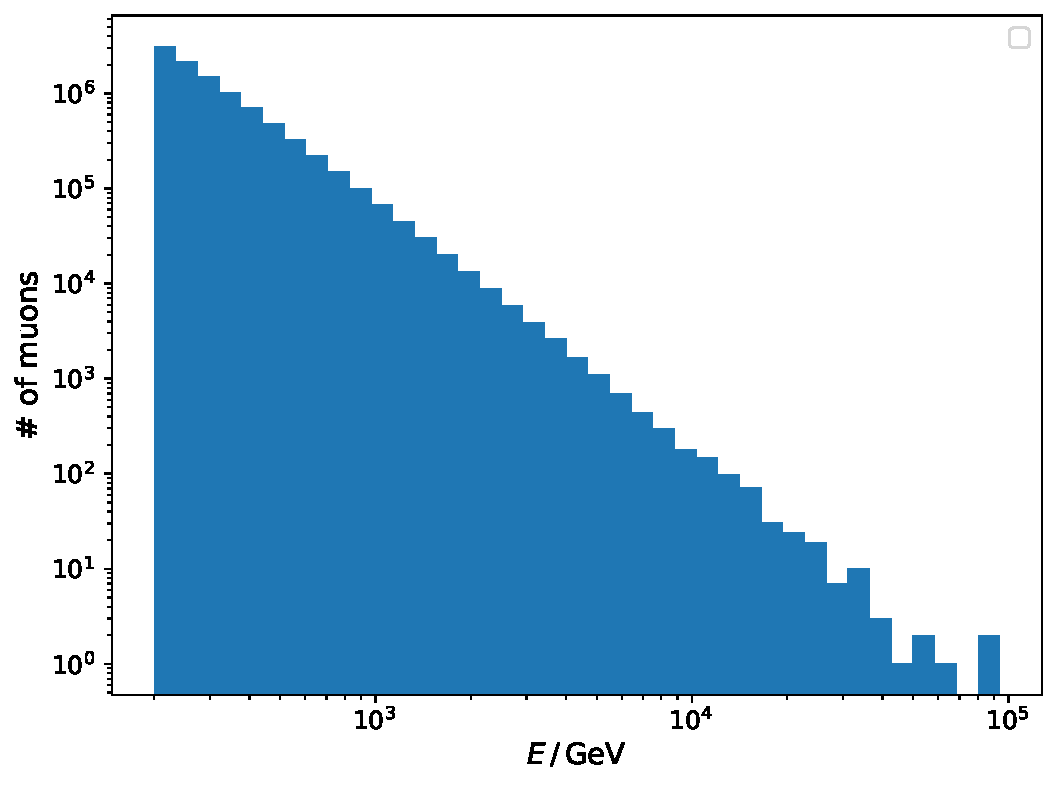
\includegraphics[width=0.7\textwidth]{Ecomug_spektrum779.pdf}
    \caption{Das verwendete Energiespektrum, mit EcoMug erzeugt.}
    \label{fig:ecomugplot}
\end{figure}


% \marktodo{ ecomug plots:
% energieverteilung mit cut
% winkelverteilung}

Zur Übertragung der Simulationsdaten auf die echte Welt, wird die 
Myonenfluss-Parametrisierung \eqref{eqn:dN_dE} über 
$E$ in den Grenzen \SI[]{600}[]{GeV} bis \SI[]{200}[]{TeV}, sowie
$\Omega$ von $0°$ bis $30°$ integriert.
Bei einer angenommenen Detektorgrundfläche von 
\SI[]{75}[]{cm^2} ergibt sich eine Myonenrate von:
\begin{align}
    \Phi_0 = 1.0857\:  \frac{\mathrm{Myonen}}{\mathrm{Tag}}.
\end{align}

Zur Berechnung der Detektorrate in Abhängigkeit zur Tiefe wird gerechnet:
\begin{equation}
    \Phi_h = \Phi_0 * a 
\end{equation}
$\Phi_h$ als Detektorrate mit dem Wasserstand $h$ und $a$ 
als der Anteil der Myonen, die es zum Detektor geschafft haben. 

Es wird angenommen, das der Detektor jedes Myon, das ihn trifft, messen kann.
Eine Detektion über die seitliches Flächen des Detektors wird nicht berücksichtigt.
Im Gegensatz zur echten Welt wird keine langsam steigende Wasserhöhe simuliert,
sondern die Messrate mehrerer statischen Wasserstände.

\begin{figure}[h]
    \centering
    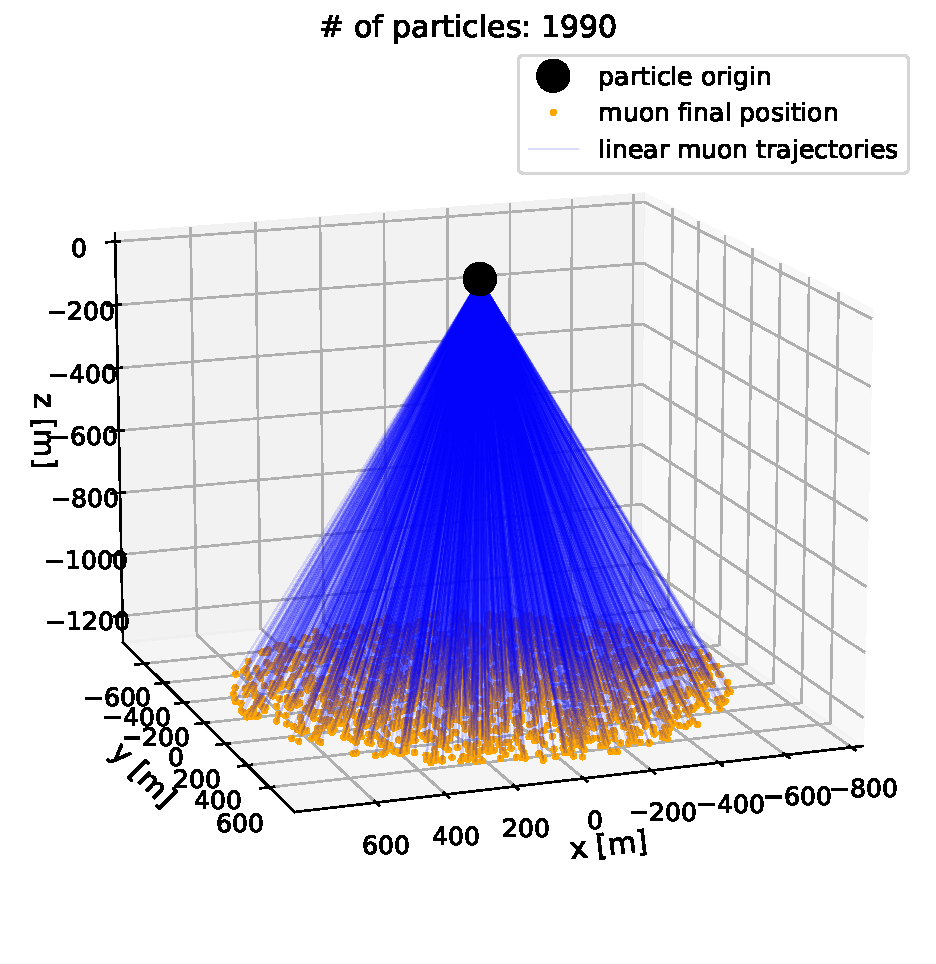
\includegraphics[width=0.7\textwidth]{plot_3D_start_end.pdf}
    \caption{Veranschaulichung der Start und Endpunkte der Myonen die den Detektor erreicht haben.
    Die Punkte werden durch eine blaue gerade Linie verbunden. 
    Alle Myonen werden bei \SI[]{1259}[]{m} gestoppt.}
    \label{fig:3d-plot}
\end{figure}
\section{Simulation der Myonen mit PROPOSAL}

PROPOSAL propagiert die Teilchen, hat allerdings gegenüber der echten Welt Einschränkungen.
Durch die Energieschnitte (siehe Kap. \ref{sec:pp-theorie}) wird ein Teil immer
kontinuierlich genähert. Durch die Wahl eines kleinen $v_\mathrm{cut}$ ist dieser Effekt 
allerdings vernachlässigbar.
Des Weiteren muss bezüglich der Messunsicherheit PROPOSALs 
bedacht sein, dass sich PROPOSAL nicht in allen Energiebereichen 
und Szenarien vergleichen kann mit echten Daten, sondern dort sich mit
ähnlichen Simulationsprogrammen vergleicht. 


\section{Ergebnisse}
% \section{Konfiguration von PROPOSAL}
\label{sec:pp-config}

Die Ergebnisse der Simulation sind in Tabelle \ref{tab:wassertiefen_tabelle} aufgelistet.
Auf den Detektor umgerechneten Detektorzählraten sind in \ref{fig:results} dargestellt.
In Abb. \ref{fig:pp_energiespekten} ist das Energiespektrum der ursprünglichen Myonen 
dieser die am Detektor angekommen sind, sowie die Endenergien am Detektor. 

Es ist ein klarer Zusammenhang zwischen Wassertiefe und Myonenanzahal bzw. Detektorrate erkennbar.
Damit ist bestätigt, sich Wassertiefen in alten Berbauregionen mithilfe der Myographie messen lassen.
% Es ist in Abb. \ref{} und \ref{} jeweils das Energiespektrum der Myonen am Detektor sowie
% deren ursprüngliches zu sehen. 
Zwischen der höchsten (\SI[]{840}[]{m}) und niedrigsten (\SI[]{0}[]{m}) Wasserhöhe
besteht in der Detektorrate ein Unterschied von
\begin{equation}
    \Delta\Phi = \SI[]{33.2 e - 3}[]{\frac{\mathrm{Myonen}}{\mathrm{Tag}}}
    \quad \mathrm{oder}\quad \SI[]{13,06}{\%}.
\end{equation}
Zwischen den extremsten Wasserschichten Schichten sinkt also die Rate um.
Pro \SI[]{100}[]{m} sind das im Mittel eine Reduktion von
\begin{align}
    \SI[]{4.0 e-3}[]{\frac{\mathrm{Myonen}}{\mathrm{Tag}}} \quad \mathrm{oder}\quad  \SI[]{1,55}[]{\%}
\end{align}
Wird nun die wesentlich dichtere Dolomit Schicht zwischen \SI[]{748}{m} und \SI[]{840}[]{m}
betrachtet wird im Kontrast zu der darunter liegenden Tonsteinschicht
, keine signifikante Änderung der Abschwächungen der Raten beobachtet.
Es ist außerdem festzustellen, dass die Dichten der Schichten 
wenig Einfluss haben auf die Änderung der Absorption bei fixen Hohlraumvolumen. 

\begin{table}[h]
    \caption{Für verschiedene Wassertiefen, die Anzahl an detektierten Myonen
     sowie deren prozentuales Verhältnis $N_\mathrm{d}/N_0$ zur Gesamtmenge an propagierten Myonen.}
    \centering\begin{tabular}{c c c}
        Wassertiefe / \si[]{m} & \# Teilchen &  \% $N_\mathrm{d}/N_0$ \\
        0   & \num{2344409} & \num{23.44} \\
        100 & \num{2303835} & \num{23.04} \\
        200 & \num{2266474} & \num{22.66} \\
        300 & \num{2227742} & \num{22.28} \\
        324 & \num{2218556} & \num{22.19} \\
        400 & \num{2192224} & \num{21.92} \\
        500 & \num{2155066} & \num{21.55} \\
        600 & \num{2118887} & \num{21.19} \\
        700 & \num{2085579} & \num{20.86} \\
        748 & \num{2070024} & \num{20.70} \\
        800 & \num{2051255} & \num{20.51} \\
        840 & \num{2038287} & \num{20.38} \\
    \end{tabular}
    \label{tab:wassertiefen_tabelle}
\end{table}

\begin{figure}[]
    \centering
    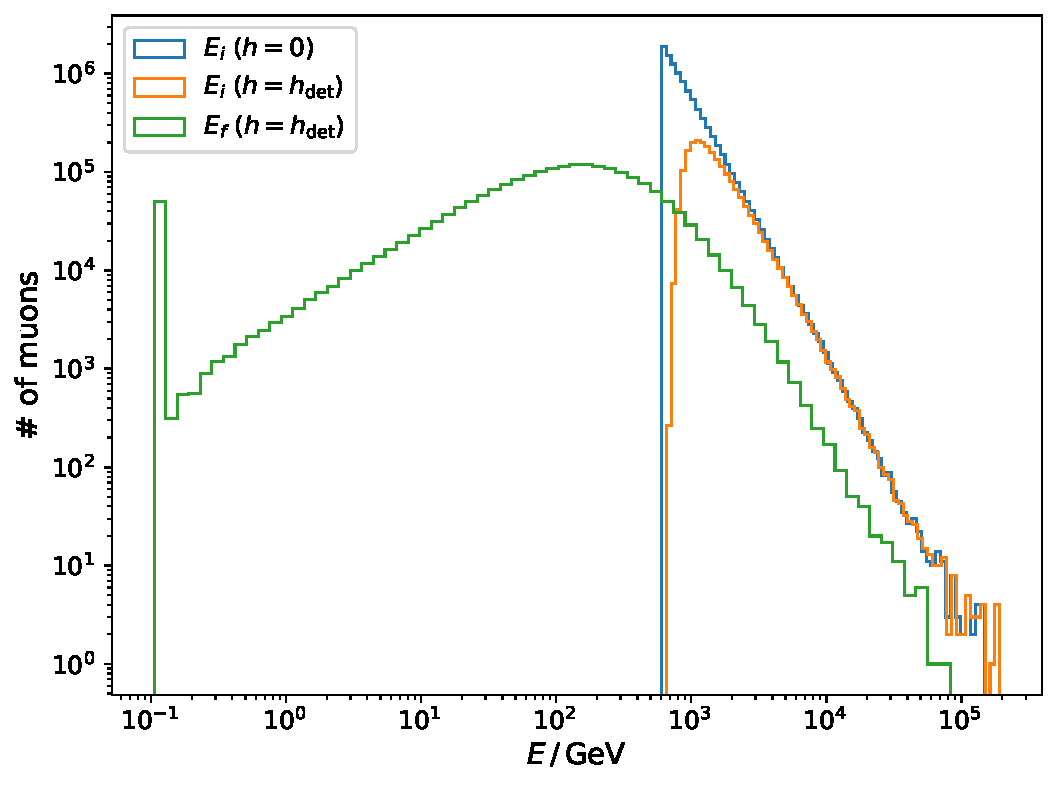
\includegraphics[width=0.8\textwidth]{EcoMug_gaisser_30deg_1e7_min6e2_max2e5.hdf_v=1.pdf}
    \caption{Das Energiespektrum für eine Wassertiefe von \SI[]{800}[]{m}.
        In Blau die ursprünglichen Myonen auf der Erdoberfläche.
        In Orange diejenigen, die angekommen sind. 
        In Grün die Endenergie der Myonen am Detektor.}
    \label{fig:pp_energiespekten}
\end{figure}


\begin{figure}[h]
    \centering
    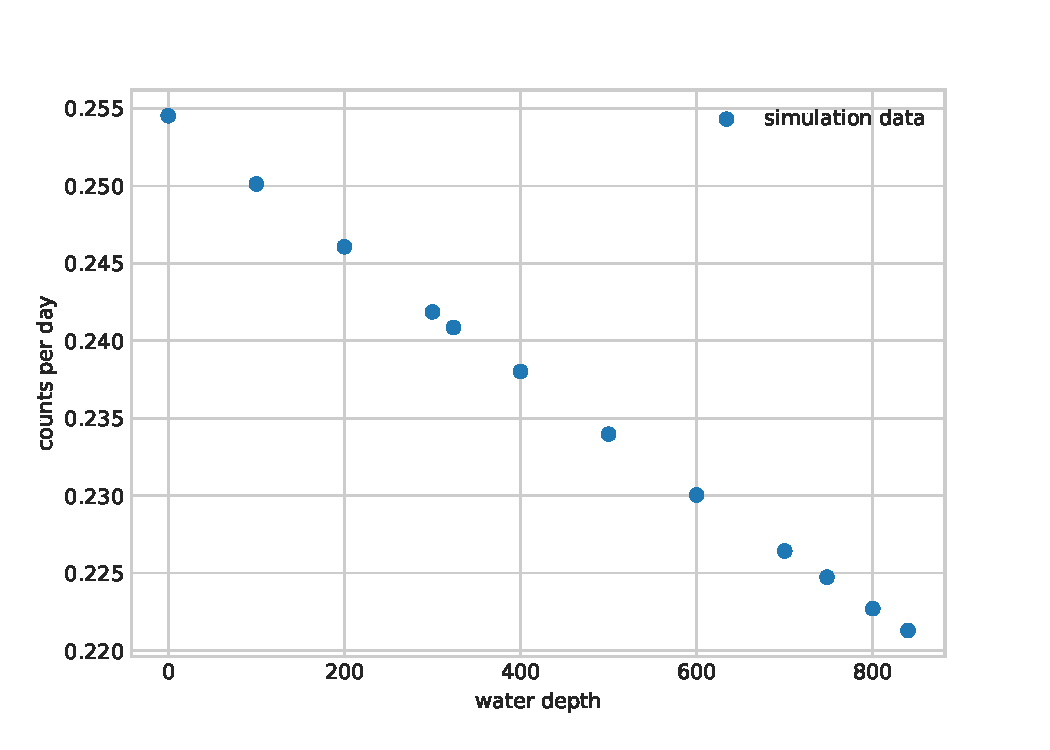
\includegraphics[width=0.8\textwidth]{results_plot.pdf}
    \caption{Detektorraten in Teilchen pro Tag gegen die 
    Wasser Tiefe.}
    \label{fig:results}
\end{figure}
\chapter{Zusammenfassung und Ausblick}

% \marktodo{Forschungsfrage beantworten und einordnen: tatsächliche Aussagekraft und Einschränkungen\\
% inwiefern sind die aussagen aus dieser arbeit übertragbar auf die realword} 
% diskussion:

In dieser Arbeit wurde anhand einer Bohrung aus dem Ruhrgebiet ein Bodenmodell erstellt,
um Detektorzählraten bei verschiedenen Wasserständen innerhalb
für den Bergbau trocken gelegten Erdschichten zu simulieren.
Es konnten signifikante Unterschiede in den Zählraten gezeigt werden.
Pro \SI[]{100}[]{m} ändert sich die Detektorrate um \SI[]{1,55}[]{\%}.

% Die ausgerechneten Messzeiten um einen Wasserstand mit einer Genauigkeit von
% \SI[]{100}[]{m} mithilfe des beschriebenen Detektor auflösen zu
% können, beträgt \SI[]{01010101}[]{Tage} .....  \marktodo{spezifizieren}

Da sich in der Realität die Wasserstände um \si[]{cm} pro Woche ändern können,
detektiert der in dieser Arbeit angenommene Detektor zu wenig Teilchen pro Tag,
um Veränderungen schnell genug oder überhaupt verlässlich nachweisen zu können.

Da in dieser Arbeit nur die Detektion über die horizontale Oberfläche in Betracht gezogen wird,
könnte in zukünftigen Arbeiten über die Vergrößerung des Detektors in vertikaler Richtung
die Messzeit gesenkt werden, technisch ist lediglich zu beachten, dass der Detektor in 
\SI[]{30}[]{Fuß} Schritten teilbar sein muss. 
Des Weiteren sollte über Alternativen zur Platzierung des Detektors innerhalb
einer Bohrung nachgedacht werden. Der Durchmesser von \SI[]{10}[]{cm} 
limitiert die Möglichkeiten des Detektors massiv.

Alte Bergwergschächte hatten ursprünglich einen Durchmesser von \num[]{7} bis \SI[]{10}[]{m}.
Dort existieren teilweise Inspektionsrohre mit einem Durchmesser von \num[]{80} bis \SI[]{100}[]{cm}.
Diese werden vorgehalten, um ggf. Pumpen einzuhängen. Jene Inspektionsrohre würden alleine durch den höheren
Durchmesser eine ca. \num[]{24} mal größere Grundfläche besitzen können, welche
bspw. die Rate für \SI[]{800}[]{m} von 
\SI[]{0.254}[]{\frac{\mathrm{Myonen}}{\mathrm{Tag}}} auf 
\SI[]{6.108}[]{\frac{\mathrm{Myonen}}{\mathrm{Tag}}} heben würde.




Wenn die xy-Ebene einer Bohrung verlassen wird, treten große Inhomogenitäten auf.
Dies senkt die Übertragbarkeit des Bodenmodells auf die echte Welt.
Um diese zu verbessern, könnten mit mehr Bohrungen das Bodenmodell in der xy-Ebene verfeinert werden,
um die Berechnung zu verbessern.

Spannend könnte im Rahmen kommender Arbeiten eine echte 
Messung innerhalb eines Bohrlochs oder anderen Öffnungen sein.
Es könnte untersucht werden, inwiefern die in dieser Arbeit bestimmten
relativen Raten-Unterschiede mit den Vorhersagen dieser Arbeit übereinstimmen.

Auch könnte ein Vergleich der absoluten Detektorraten mit den simulierten
ein Maß über die Gültigkeit aller Näherungen in dieser Arbeit liefern. 

% energiethreshold zur verbesserung der aussaagekraft

% \input{content/00_abstr.tex} nicht notwendig
% \input{content/04_res.tex}

\appendix
% Hier beginnt der Anhang, nummeriert in lateinischen Buchstaben
\chapter{Anhang}


\section{verwendete Programme}

Der Programmcode dieser Arbeit ist unter 
\url{https://github.com/Martin-SF/muography-bachelor}
verfügbar.

Alle Ergebnisse werden mit Python 3.10.4 (\url{https://www.python.org})
mit Hilfe dieser aufgelisteten Bibliotheken erzeugt:
\begin{enumerate}
    \item PROPOSAL 7.3.1 (\url{https://github.com/tudo-astroparticlephysics/PROPOSAL})
    \item EcoMug 1.3.1 (\url{https://github.com/dr4kan/EcoMug})
    \item Numpy 1.21.6 (\url{https://numpy.org/})
    \item pandas 1.4.2 (\url{https://pandas.pydata.org/})
    \item matplotlib 3.5.2 (\url{https://matplotlib.org/})
    \item distributed 2022.5.0 (\url{https://distributed.dask.org/en/stable/})
    \item tqdm 4.64.0 (\url{https://github.com/tqdm/tqdm})
    \item numba 0.55.1 (\url{https://numba.pydata.org/})
    \item pytables 3.7.0 (\url{https://www.pytables.org/})
    \item prettytable 3.2.0 (\url{https://pypi.org/project/prettytable/})
    \item scipy 1.8.0 (\url{https://scipy.org/})
    \item uncertainties 3.1.6 (\url{https://pythonhosted.org/uncertainties/})
\end{enumerate}

%  \marktodo{standort in eigenes figure} 
\section{Schichtverzeichnis}
\label{sec:alle_schichten}
\begin{figure}
    \centering
    % 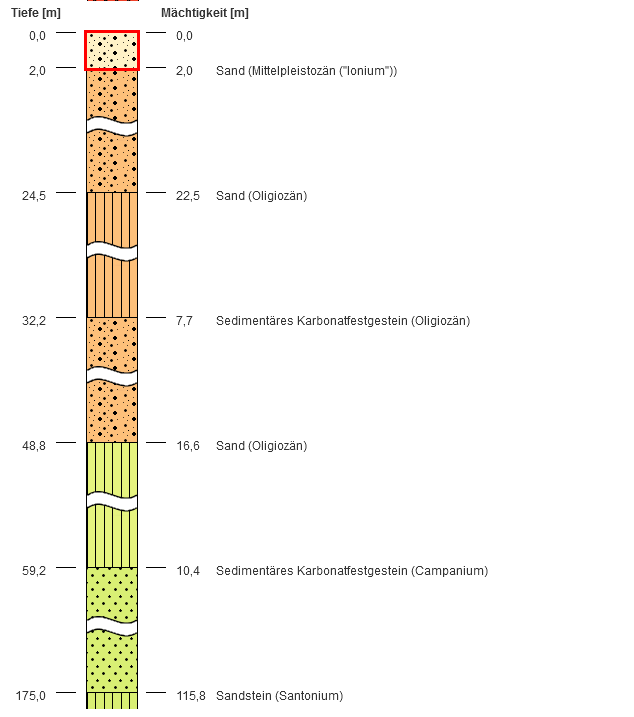
\includegraphics[width=0.49\textwidth]{schichtverzeichnis_1.png}
    % 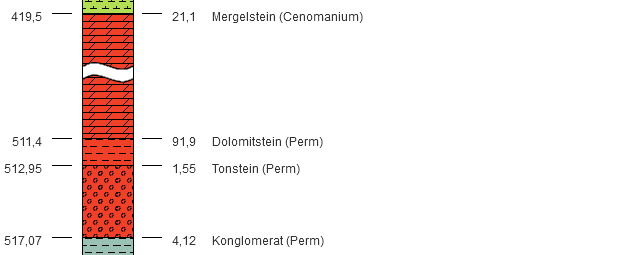
\includegraphics[width=0.49\textwidth]{schichtverzeichnis_3.png}
    % 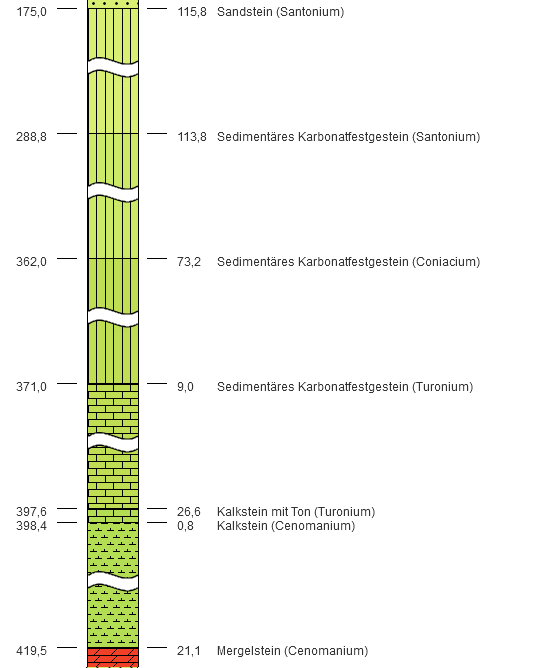
\includegraphics[width=0.49\textwidth]{schichtverzeichnis_2.png}
    % 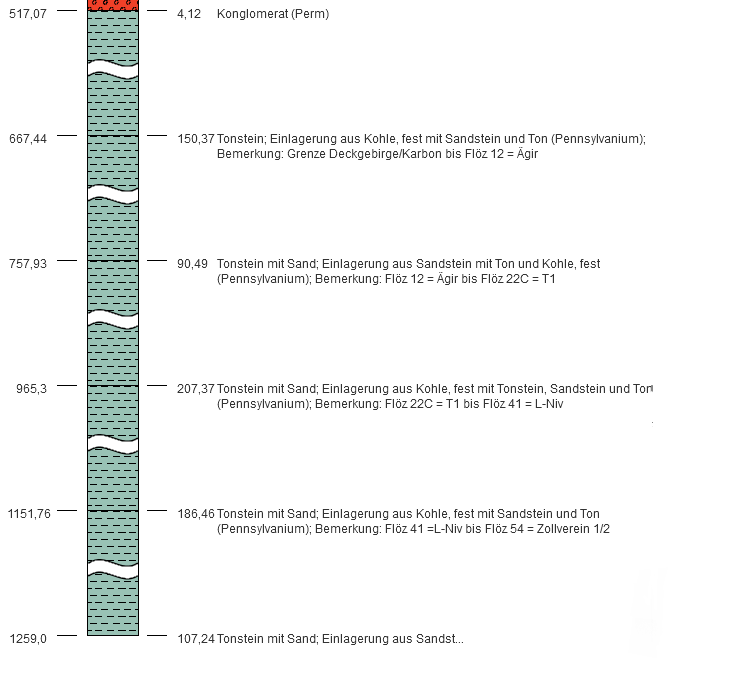
\includegraphics[width=0.49\textwidth]{schichtverzeichnis_4.png}
    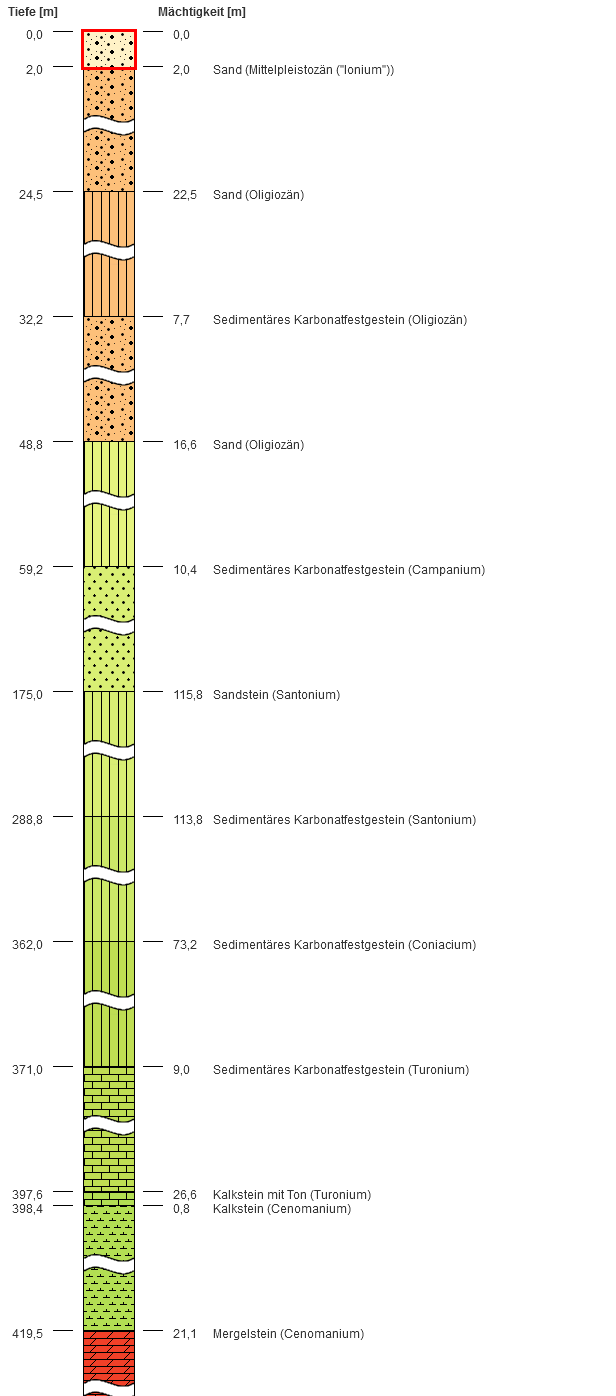
\includegraphics[width=0.49\textwidth]{schichtverzeichnis_10.png}
    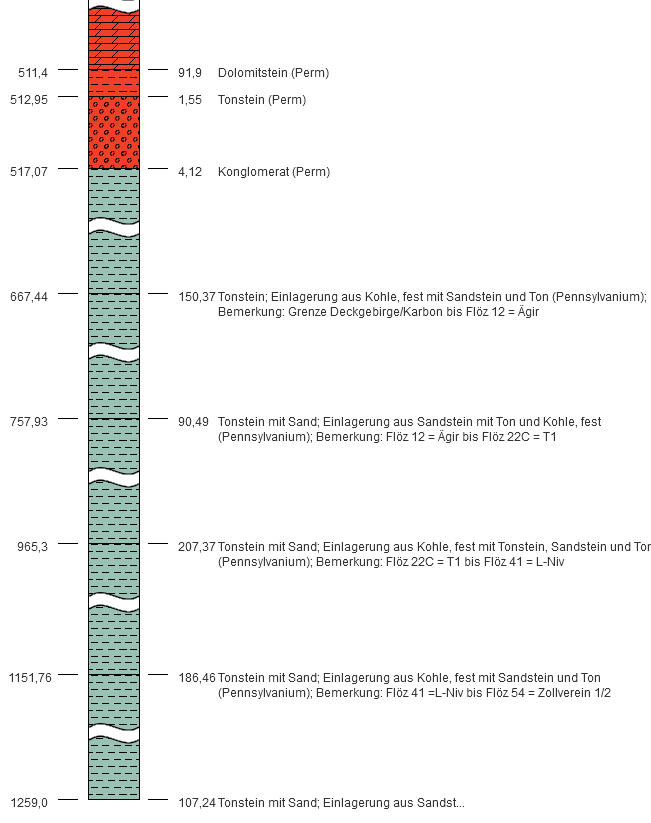
\includegraphics[width=0.49\textwidth]{schichtverzeichnis_11.png}
    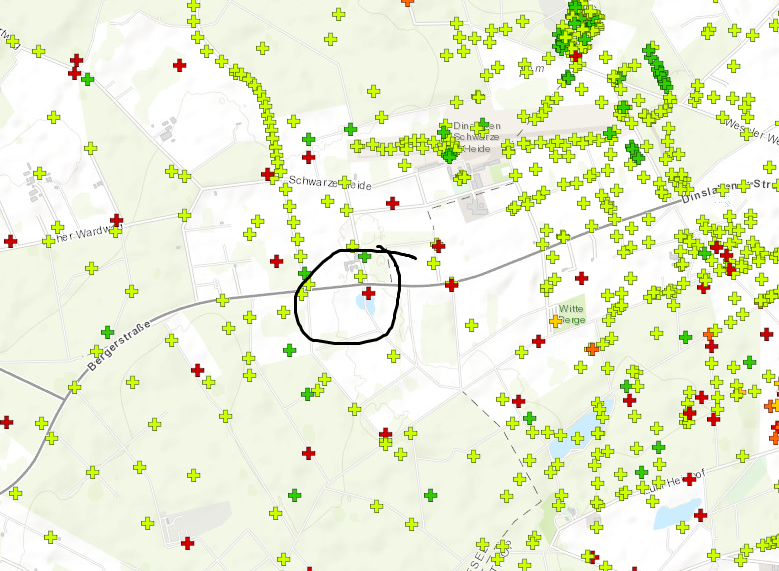
\includegraphics[width=0.49\textwidth]{schichtverzeichnis_location.png}
    \caption{Zu sehen sind die einzelnen Schichten einer Bohrung nahe
     Bottrop. Die erste Zahl steht für die Tiefe des unteren Ende der Schicht in \si[]{m}, die zweite 
    Zahl ist die Dicke der Schicht in \si[]{m}. Der Standort ist im untersten Bild markiert. Zu finden unter 
    \url{boreholemap.bgr.de/mapapps/resources/apps/boreholemap/}. 
    Standort: (\num[]{351221,19} \num[]{5719599,6}) 
    ID: DABO\_65808 (nahe dem Schwarze Heide Airport)}
    \label{fig:Schichtverzeichnis_komplett}
\end{figure}





\section{Konfiguration von EcoMug}
Für EcoMug ist ein Pythoninterface erstellt worden
\footnote{pybind11\url{https://github.com/pybind/pybind11}}. Alle relevanten Funktionen EcoMugs sind nun also auch aus Python benutzbar.
Energieangaben sind in EcoMug immer als Impuls des Teilchens definiert. Zur Vereinheitlichung werden alle
Werte EcoMugs in die Schwerpunktsenergie umgerechnet. 
Mit Dask.distributed wird die Erzeugung der Myonen auf
mehrere Kerne parallelisiert. Jeder Kern zieht einen eigenen zufälligen Seed für EcoMug.

Während erster Testläufe wird festgestellt, dass die in EcoMug standardmäßig verwendete 
Parametrisierung für den Myonenfluss auf Meereshöhe nicht für hohe Energien geeignet ist.


% Es wird aus \cite[]{Alexandrov2017} der Plot aus Abb. \(\)

%  \marktodo{ ändern} 
% Dies ist in Abb. \ref{todo} aus \cite[]{Alexandrov2017} mit EcoMugs Standard
% Parametrisierung erstellt, zu sehen in Abb. \ref{todo}.

% % todo figure fig 4
%  \marktodo{todo} In Abb. \ref{fig:} ist zu sehen wie in Abhängigkeit zu $\cos\theta$ (Zenit Winkel),
% die Energie sinkt.


%  \marktodo{$\theta \leq 30°$ erklären/motivieren.} 
% Es wird zwar EcoMug auf $\theta \leq 30°$ konfiguriert siehe Sektion \ref{sec:pp-config}, 
% dennoch ist selbst für diesen Bereich eine Abweichung zu sehen.
%  \marktodo{andere plots von std vs gaisser wo sich die unterschiede deutlicher zeigen}  

 In Testläufen ergibt sich eine Menge von 
\num{e7} Myonen als geeignetes Mittelmaß zwischen Präzision und 
Laufzeit
Auf dem \textit{phobos} Server des Lehrstuhls benötigt 
EcoMug ca. eine Minute und PROPOSAL ca. \SI[]{30}[]{min} um 10 Mio. Myonen zu generieren bzw. zu propagieren
pro Wassertiefe. Specs: 2x Intel(R) Xeon(R) CPU E5-2680 v3 @ 2.50GHz (je 12 Kerne); 128 GB RAM.

Außerdem ergibt sich, dass Myonen min. über \SI[]{600}[]{GeV} je nach Wasserstand 
brauchen, um den Detektor erreichen zu können.
Bei \SI[]{8}[]{m} Wasserstand haben Myonen mit der geringsten Energie \SI[]{638.9}[]{GeV} (\num[]{1e7} 
simulierte Myonen)
Aufgrund dessen wird in EcoMug die minimale Myonenenergie auf \SI[]{600}[]{GeV} gesetzt.

Ohne diesen Energieschnitt haben die hochenergetischsten Myonen bei \num{e7} erzeugten
ca. \SI[]{200}[]{GeV} wie in Abb. \ref{fig:minenergieplot} zu sehen.

% oberhalb von \SI[]{800}[]{GeV}, nun sind es mit der Anpassung einstellige Prozentbereiche.
%  \marktodo{kleiner machen, mit anderem plot vereinen} 

\begin{figure}[h]
    \centering
    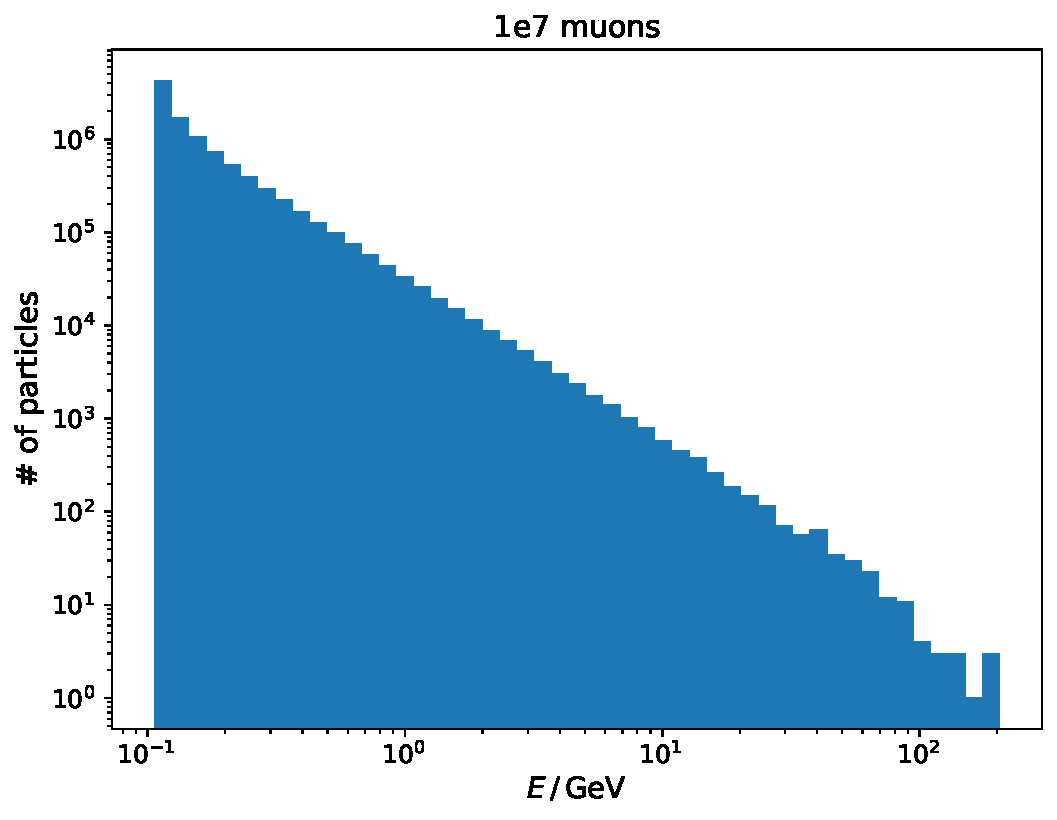
\includegraphics[width=0.7\textwidth]{1e7 muons.pdf}
    \caption{10 Mio. Myonen mit EcoMug (Gaisser) ohne Energieschnitt erzeugt.
    Die maximale Energie liegt lediglich bei ca. \SI[]{200}[]{GeV}. }
    \label{fig:minenergieplot}
\end{figure}

In Testläufen mit \num{e7} Myonen ergibt sich wie in Abb. \ref{fig:ecomugplot} zu sehen,
dass die hochenergetischsten Myonen unter \SI[]{100}[]{TeV} bleiben.

Deshalb wird die maximale Myonenenergie in EcoMug auf \SI[]{200}[]{TeV} gesetzt. 
\footnote{Der Grund dafür ist, dass EcoMugs Laufzeit mit der Breite des Energiebereichs skaliert. 
Es sollte also ein Energiemaximum leicht oberhalb des maximalen $E_\mu$ gewählt werden.}  

% restliche Konfiguration#
Des Weiteren wird die Generationsfläche auf einen Punkt vereinfacht (siehe Kap. \ref{sec:pp-config}),
d.h. jedes Myon hat als Start Position
(0,0,0)\footnote{
    Zur Vermeidung unnötiger Zyklen wird im gesamten Programmcode
    angenommen das die Myonen bei (0,0,0) starten.}
Im Abschnitt \ref{sec:pp-config}
findet sich die Begründung.


\section{Konfiguration von PROPOSAL}

Da das erstellte Bodenmodell eindimensional ist und die verwendete Gaisser-Parametrisierung
(siehe Kap. \ref{sec:myonenfluss}) $\theta < 70°$ vorschreibt, da es die Erdkrümmung
vernachlässigt, wird sich folgende Näherung überlegt:
Es wird die Emissionsfläche der Myonen mit dem, in der Größenordnung des Experiments 
punktförmigen Detektor, vertauscht.
Diese Näherung garantiert das jedes Myon, soweit es genug Energie besitzt, den Detektor trifft.
% Dies ist die Optimierung mit der höchsten Laufzeit Verbesserung in dieser Arbeit.

Zu den in Kap. \ref{sec:bodenmodell} beschriebenen Schichten wird der PROPOSAL 
Konfiguration noch eine Detektorschicht hinzugefügt und eine \textit{hierarchy}
von 20 gegeben. Die \textit{hierarchy}-Bedingung wird dazu benutzt zu definieren, 
wann PROPOSAL mit der Propagation stoppen soll.
Diese Schicht repräsentiert ohne die am 
Anfang des Kapitels beschriebene Näherung anschaulich die Fläche der Myonen aus der Atmosphäre,
welche den Detektor treffen. 

% Zur Auswahl des Energy-Cuts und der Vielfachstreuung werden Tests gemacht,
% dessen Ergebnisse in Abb. \ref{fig:cut_scat_tests} zu sehen sind.

% \marktodo{fig} 
% \begin{figure}[h]
%     \centering
%     \includegraphics{}
%     \caption{Zu sehen die Anzahl an Myonen, die an einem Detektor in \SI[]{1205}[]{m}}
%     angekommen sind, in Abhängigkeit zu $v_\mathrm{cut}$ und verschiedene Vielfachstreuungen.}
%     \label{fig:cut_scat_tests}
% \end{figure}

Für die Berechnung der Ergebnisse wird folgende Konfiguration verwendet:
\begin{align}
    v_\mathrm{cut} = 0.001  \;\; \mathrm{und} \;\; \mathrm{multiplescattering} = \mathrm{Highland}
\end{align}

% Zur finalen Propagation lädt PROPOSAL die von EcoMug erzeugten Myonen aus einer HDF5-Datei.
% Es wird Teilchenart, Energie und Richtung ausgelesen. Die Position wird für jedes Teilchen statisch
% auf (0,0,0) gesetzt.
% Nun propagiert PROPOSAL bis zum Zerfall des Teilchens oder bis es den Detektor erreicht hat.
% Dazu wird aus dem \textit{track}-Objekt welches PROPOSAL als Ergebnis ausgibt, 
% die $z$-Koordinate ausgelesen verglichen mit der des Detektor-Sektors.
% Hat das Myon den Detektor erreicht, wird 
% der  \marktodo{output } in eine HDF5-Datei gespeichert. Der Name der Datei enthält außerdem
%  die Anzahl an Myonen die insgesamt propagiert wurden.

 Zur weiteren Optimierung der Laufzeit wird wieder mit Dask.distributed 
 eine Parallelisierung auf mehreren Kernen ermöglicht. Da PROPOSAL einen standardmäßigen
 Seed setzt erzeugt sich jeder Kern einen neuen zufälligen Seed.

\backmatter
\printbibliography
\chapter*{Danksagung}
An dieser Stelle möchte ich einigen Personen danken, ohne die diese Arbeit nicht
möglich gewesen wäre.

Zunächst danke ich Herrn Prof. Dr. Dr. Rhode sehr herzlich
für das Erstgutachten und die Möglichkeit, meine Bachelorarbeit am Lehrstuhl EVb
schreiben zu können. Herrn Prof. Dr. Kröninger möchte ich ebenfalls herzlich für das
Zweitgutachten danken. 
Ganz besonders möchte ich in erster Linie 
Jean-Marco, Pascal, Jan und Alexander der PROPOSAL Gruppe danken.
Egal an wen ich mich von euch gewandt habe, standet ihr mir immer
tatkräftig und ausdauernd an meiner Seite, auch zu ungewöhnlichen Tageszeiten.
Außerdem möchte ich mich bei Prof. Dr. Ing. Tobias Rudolph bedanken.
Sie haben uns eine Bohrung zur Verführung gestellt sowie detailliert
viele Fragen zur Geologie und Bergbau erklärt. Ohne ihr Mitwirken wäre 
diese Arbeit nicht möglich gewesen.
Des Weiteren möchte ich Mirco Hünnefeld und Dominik Baak 
für die Verbesserungsvorschläge in Bezug auf Optimierung des Codes
, sowie dem gesamten Lehrstuhl für die angenehme Atmosphäre danken.
Darüber hinaus möchte ich besonders allen aus der PROPOSAL 
Gruppe sowie meinen Freunden Sebastian, Santosh, Judith, Noah
sowie meinen Eltern für das Korrekturlesen danken,
ohne euch wäre die Arbeit nicht im Ansatz da, was sie jetzt ist.
Zum Schluss möchte ich noch meiner Familie und meinen Freunden danken, die mich in den stressigen Phasen immer wieder ermuntert haben und unterstützend
zur Seite standen.


% \cleardoublepage
% \incgraph[documentpaper][width=\paperwidth]{graphics/eidstatt.png}
\end{document}
